\subsection{Tipologia di utenti}
Prima di procedere con l’elenco degli Use Case, vengono specificati i tipi di utenti che possono interagire con l'applicazione.
\begin{figure}[h!] 
\centering 
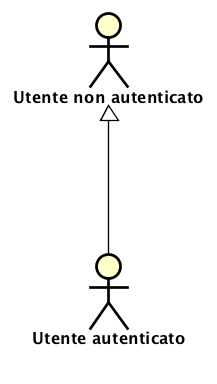
\includegraphics[scale=0.5]{../../Casi D'uso/TipologiaUtenti.png} 
\caption{Gerarchia degli utenti} 
 \end{figure} 
 
 Descrizione degli utenti:
 
 \begin{itemize}
 \item \textbf{Utente non autenticato}: è un utente che posside un account, ma deve ancora effettuare l'autenticazione; oppure un utente che intende effettuare la registrazione per poi autenticarsi.
 \item \textbf{Utente autenticato}: è un utente che ha effettuato l'autenticazione e che può utilizzare le funzionalità dell'applicazione.
 \end{itemize}
 
\subsection{Notazione Use Case}
L'analisi del capitolato, l'incontro con Zucchetti S.r.l. e la discussione tra gli \emph{Analisti} ha portato alla definizione dei seguenti casi d'uso.\\
Ogni caso d’uso presente ha un codice univoco gerarchico, nella forma:
\[UC[codice del padre].[codice progressivo di livello]\]
Il codice progressivo puoò includere diversi livelli di gerarchia separati da un punto.

\newpage
\subsection{UC0 - Visione Generale} 
\label{ssec:UC0} 
\begin{figure}[h!] 
\centering 
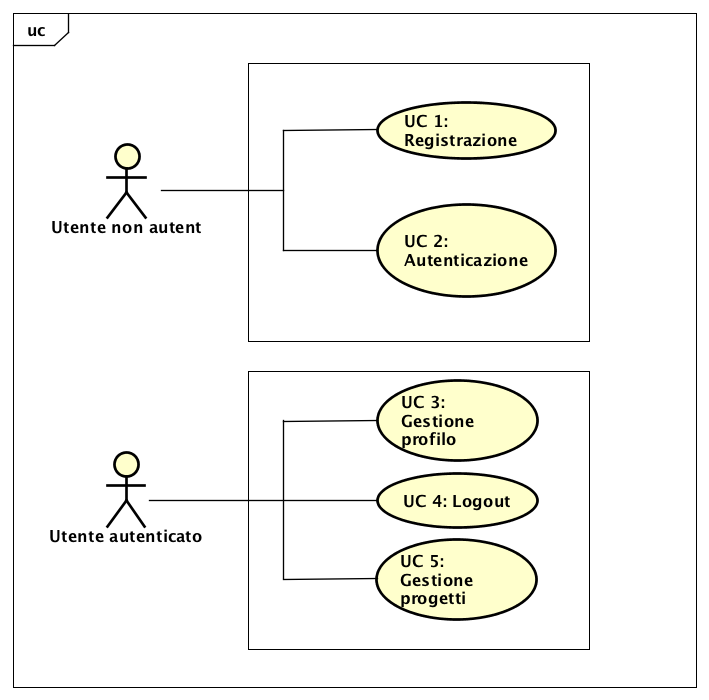
\includegraphics[scale=0.5]{../../Casi D'uso/Generale.png} 
\caption{Caso d'uso UC0} 
 \end{figure} 
\begin{itemize} 
\item \textbf{Attori}: Utente non autenticato e Utente autenticato;
\item \textbf{Descrizione}: Vengono visualizzate in generale le vari funzionalità che l'applicazione permette ai vari utenti di svolgere;
\item \textbf{Precondizione}: L'applicazione predispone l'interazione con un attore, facendolo accedere alle diverse funzionalità proposte;
\item \textbf{Postcondizione}: Dopo l'interazione avvenuta con un attore, l'applicazione si troverà in un nuovo stato pronto ad interagire con un nuovo attore;
\item \textbf{Scenario principale}: \begin{enumerate}\item Registrazione (UC1);\item Autenticazione (UC2);\item Gestione profilo(UC3);\item Logout (UC4);\item Gestione progetti (UC5);\item Tool Designer (UC6);
 \end{enumerate}
\end{itemize} 

\subsection{UC1 - Registrazione} 
\label{ssec:UC1} 
\begin{figure}[h!] 
\centering 
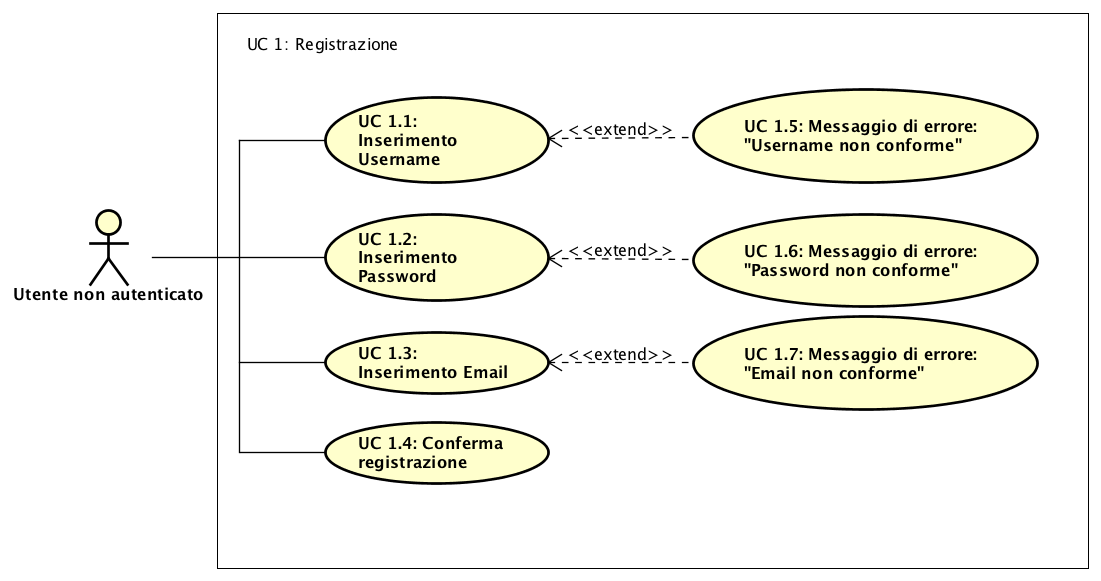
\includegraphics[scale=0.5]{../../Casi D'uso/UC1.png} 
\caption{Caso d'uso UC1} 
 \end{figure} 
\begin{itemize} 
\item \textbf{Attori}: Utente non autenticato;
\item \textbf{Descrizione}: L'attore desidera effettuare l'operazione di registrazione. Vengono richiesti dall'applicazione un username, univoco e conforme alle richieste, una password conforme alle richieste e una mail che rispetti il pattern predefinito;
\item \textbf{Precondizione}: L'applicazione predispone la possibilità di registrazione;
\item \textbf{Postcondizione}: L'applicazione ha creato un nuovo account utente;
\item \textbf{Scenario principale}: \begin{enumerate}\item Inserimento Username (UC1.1);\item Inserimento Password (UC1.2);\item Inserimento Email (UC1.3);\item Conferma registrazione (UC1.4).
\end{enumerate}
\item \textbf{Scenari alternativi}: 
	\begin{itemize}
	\item Messaggio di errore: "Username non conforme" (UC1.5);\item Messaggio di errore: "Password non conforme" (UC1.6);\item Messaggio di errore: "Email non conforme" (UC1.7). 
	\end{itemize}
\end{itemize} 
\subsection{UC1.1 - Inserimento Username} 
\label{ssec:UC1.1} 
\begin{itemize} 
\item \textbf{Attori}: Utente non autenticato;
\item \textbf{Descrizione}: L’attore inserisce l'username: deve essere univoco all'interno dell'applicazione e deve essere alfanumerico;
\item \textbf{Precondizione}: L'applicazione è pronta e l'attore intende autenticarsi;
\item \textbf{Postcondizione}: L'applicazione ha l’informazione relativa all'email inserita dall’attore.
\end{itemize} 
\subsection{UC1.2 - Inserimento Password} 
\label{ssec:UC1.2} 
\begin{itemize} 
\item \textbf{Attori}: Utente non autenticato;
\item \textbf{Descrizione}: L’attore inserisce la password: deve essere di tipo alfanumerico e può contenere caratteri di punteggiatura.;
\item \textbf{Precondizione}: L'attore intende effettuare la registrazione inserendo la password.;
\item \textbf{Postcondizione}: L'attore ha inserito una password conforme alle richieste dell'applicazione.
\end{itemize} 
\subsection{UC1.3 - Inserimento Email} 
\label{ssec:UC1.3} 
\begin{itemize} 
\item \textbf{Attori}: Utente non autenticato.
\item \textbf{Descrizione}: L’attore inserisce l'email per effettuare la registrazione;
\item \textbf{Precondizione}: L'attore ha selezionato l'opzione di registrazione e non ha ancora inserito un email;
\item \textbf{Postcondizione}: L'applicazione ha l’informazione relativa alla password inserita dall’utente;
\end{itemize} 
\newpage
\subsection{UC1.4 - Conferma registrazione} 
\label{ssec:UC1.4} 
\begin{itemize} 
\item \textbf{Attori}: Utente non autenticato;
\item \textbf{Descrizione}: Dopo che un attore ha effettuato correttamente una registrazione, ne viene informato;
\item \textbf{Precondizione}: L'attore ha scelto di effettuare l'operazione di registrazione;
\item \textbf{Postcondizione}: L'attore ha ricevuto un messaggio di conferma dell'avvenuta registrazione.
\end{itemize} 
\subsection{UC1.5 - Messaggio di errore: "Username non conforme"} 
\label{ssec:UC1.5} 
\begin{itemize} 
\item \textbf{Attori}: Utente non autenticato;
\item \textbf{Descrizione}: L'attore può inserire un username non conforme e gli viene quindi comunicato l'errore;
\item \textbf{Precondizione}: L'applicazione è pronta e l'utente intende registrarsi;
\item \textbf{Postcondizione}: L'attore ha inserito un username non conforme e ha ricevuto la comunicazione dell'errore.
\end{itemize} 
\subsection{UC1.6 - Messaggio di errore: "Password non conforme"} 
\label{ssec:UC1.6} 
\begin{itemize} 
\item \textbf{Attori}: Utente non autenticato;
\item \textbf{Descrizione}: L'attore può inserire una password non conforme e gli viene quindi comunicato l'errore;
\item \textbf{Precondizione}: L'applicazione è pronta e l'utente intende registrarsi;
\item \textbf{Postcondizione}: L'attore ha inserito una password non conforme e ha ricevuto la comunicazione dell'errore.
\end{itemize} 
\subsection{UC1.7 - Messaggio di errore: "Email non conforme"} 
\label{ssec:UC1.7} 
\begin{itemize} 
\item \textbf{Attori}: Utente non autenticato;
\item \textbf{Descrizione}: L'attore può inserire un'email con una sintassi non valida e gli viene quindi comunicato l'errore;
\item \textbf{Precondizione}: L'applicazione è pronto e l'utente intende registrarsi;
\item \textbf{Postcondizione}: L'attore ha inserito un'email non conforme e ha ricevuto la comunicazione dell'errore.
\end{itemize} 
\newpage
\subsection{UC2 - Autenticazione} 
\label{ssec:UC2} 
\begin{figure}[h!] 
\centering 
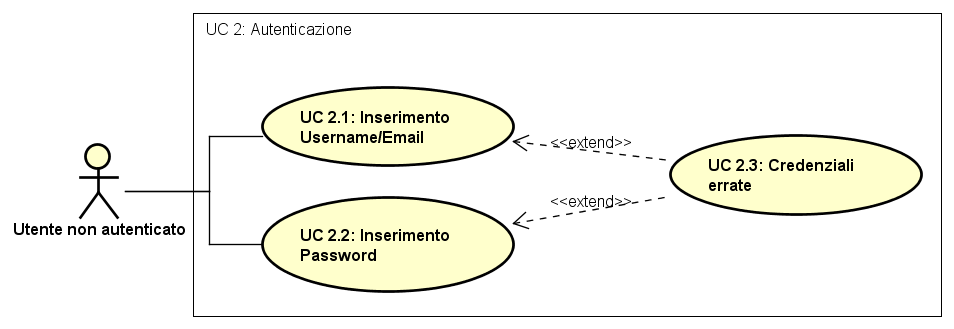
\includegraphics[scale=0.5]{../../Casi D'uso/UC2.png} 
\caption{Caso d'uso UC2} 
 \end{figure} 
\begin{itemize} 
\item \textbf{Attori}: Utente non autenticato;
\item \textbf{Descrizione}: L'attore che già in possesso delle credenziali per accedere all'applicazione, potrà effettuare l'operazione di autenticazione inserendo l'email/username e la password. Nel caso l’attore abbia perso la password o se la sia dimenticata, l'applicazione fornisce la possibilità di averne una temporanea per poi resettarla;
\item \textbf{Precondizione}: L'attore decide di autenticarsi e l'applicazione richiede l'inserimento dei dati necessari per l'autenticazione;
\item \textbf{Postcondizione}: L'attore ha avuto accesso alle funzionalità del l'applicazione, in caso l'autenticazione sia avvenuta con successo, altrimenti viene visualizzato un messaggio d'errore.
\item \textbf{Scenario principale}: \begin{enumerate}\item Inserimento Username/Email (UC2.1);\item Inserimento Password (UC2.2);\item Password dimenticata (UC2.3);  \end{enumerate}

\item \textbf{Scenari alternativi}: \begin{enumerate}
\item Credenziali errate (UC2.4);\item Invio password per email (UC2.5). \end{enumerate}

\end{itemize} 
\subsection{UC2.1 - Inserimento Username/Email} 
\label{ssec:UC2.1} 
\begin{itemize} 
\item \textbf{Attori}: Utente non autenticato;
\item \textbf{Descrizione}: Durante la fase di autenticazione viene richiesto all'attore il proprio username oppure la propria email;
\item \textbf{Precondizione}: L'applicazione è pronta e l'attore intende autenticarsi;
\item \textbf{Postcondizione}: L'applicazione ha l’informazione relativa all'email/username inserita dall’attore.
\end{itemize} 
\subsection{UC2.2 - Inserimento Password} 
\label{ssec:UC2.2} 
\begin{itemize} 
\item \textbf{Attori}: Utente non autenticato;
\item \textbf{Descrizione}: Durante la fase di autenticazione viene richiesta all'attore la propria password;
\item \textbf{Precondizione}: L'applicazione è pronta e l'attore intende autenticarsi;
\item \textbf{Postcondizione}: L'applicazione ha l’informazione relativa alla password inserita dall’attore.
\end{itemize} 
\subsection{UC2.3 - Password dimenticata} 
\label{ssec:UC2.3} 
\begin{itemize} 
\item \textbf{Attori}: Utente non autenticato;
\item \textbf{Descrizione}: L'attore ha smarrito la password e l'applicazione può fornirgliene una temporanea;
\item \textbf{Precondizione}: L'attore possiede un account all'interno dell'applicazione, ma non è più in possesso della password;
\item \textbf{Postcondizione}: L'attore ha ricevuto una email contenente la nuova password temporanea.
\end{itemize} 
\subsection{UC2.4 - Credenziali errate} 
\label{ssec:UC2.4} 
\begin{itemize} 
\item \textbf{Attori}: Utente non autenticato;
\item \textbf{Descrizione}: L’attore visualizza un messaggio di errore dato dall’inserimento di credenziali errate;
\item \textbf{Precondizione}: L'applicazione ha verificato le credenziali inserite dall’attore;
\item \textbf{Postcondizione}: L'applicazione predispone la visualizzazione di un messaggio di errore.
\end{itemize} 
\subsection{UC2.5 - Invio password per email} 
\label{ssec:UC2.5} 
\begin{itemize} 
\item \textbf{Attori}: Utente non autenticato;
\item \textbf{Descrizione}: Viene inviata una password temporanea all'attore per permettergli di accedere all'applicazione;
\item \textbf{Precondizione}: L'attore richiede una password temporanea;
\item \textbf{Postcondizione}: L'applicazione ha inviato all'attore una mail contenente la password temporanea.
\end{itemize} 
\newpage
\subsection{UC3 - Gestione Profilo} 
\label{ssec:UC3} 
\begin{figure}[h!] 
\centering 
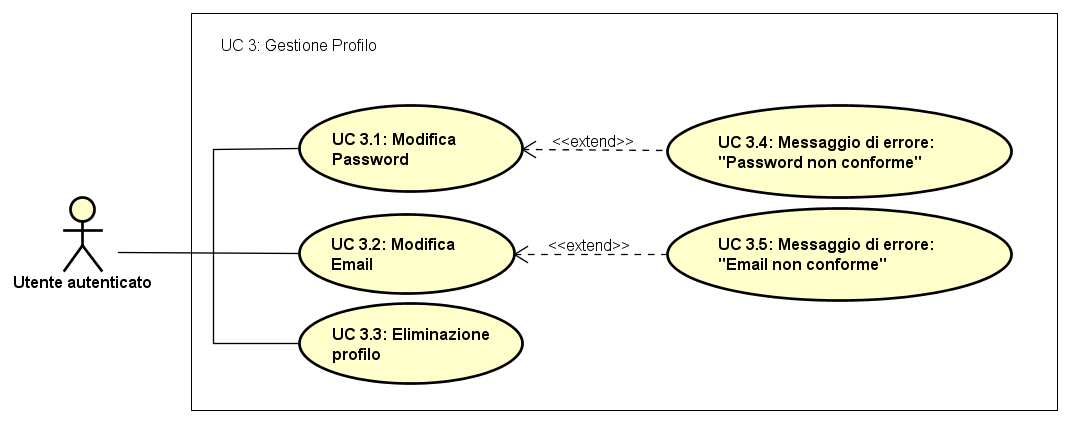
\includegraphics[scale=0.5]{../../Casi D'uso/UC3.png} 
\caption{Caso d'uso UC3} 
 \end{figure} 
\begin{itemize} 
\item \textbf{Attori}: Utente autenticato;
\item \textbf{Descrizione}: L'attore può gestire il suo username, la sua password o il suo indirizzo email;
\item \textbf{Precondizione}: L'attore ha già effettuato l'accesso e l'applicazione rende disponibile la voce Gestione Profilo nel menù;
\item \textbf{Postcondizione}: L'applicazione visualizza i dati dell'attore con gli opportuni pulsanti di modifica;
\item \textbf{Scenario principale}: 
	\begin{enumerate}\item Modifica Username (UC3.1);\item Modifica Password (UC3.2);\item Modifica Email (UC3.3);\item Eliminazione Profilo (UC3.4);\end{enumerate}
\item \textbf{Scenario alternativo}: 
	\begin{enumerate} \item Messaggio di errore: "Username non conforme" (UC3.5);\item Messaggio di errore: "Password non conforme" (UC3.6);\item Messaggio di errore: "Email non conforme" (UC3.7). 
	\end{enumerate}
\end{itemize} 
\subsection{UC3.1 - Modifica Username} 
\label{ssec:UC3.1} 
\begin{itemize} 
\item \textbf{Attori}: Utente autenticato;
\item \textbf{Descrizione}: L'attore può modificare il suo username;
\item \textbf{Precondizione}: L'attore vuole modificare l'username;
\item \textbf{Postcondizione}: L'applicazione modifica l' username dell'attore;
\item \textbf{Scenari alternativi}: L'attore annulla la modifica dell'username.
\end{itemize} 
\subsection{UC3.2 - Modifica Password} 
\label{ssec:UC3.2} 
\begin{itemize} 
\item \textbf{Attori}: Utente autenticato;
\item \textbf{Descrizione}: L'attore ha la possibilità di modificare la sua password;
\item \textbf{Precondizione}: L'attore vuole modificare la password;
\item \textbf{Postcondizione}: L'applicazione modifica la password o restituisce il messaggio d'errore;
\item \textbf{Scenari alternativi}: L'attore annulla la modifica della password.
\end{itemize} 
\subsection{UC3.3 - Modifica Email} 
\label{ssec:UC3.3} 
\begin{itemize} 
\item \textbf{Attori}: Utente autenticato;
\item \textbf{Descrizione}: L'attore ha la possibilità di modificare la propria email;
\item \textbf{Precondizione}: L'attore vuole modificare l'email;
\item \textbf{Postcondizione}: L'applicazione aggiorna l'email;
\item \textbf{Scenari alternativi}: L'attore annulla la modifica dell'email.
\end{itemize} 
\subsection{UC3.4 - Eliminazione Profilo} 
\label{ssec:UC3.4} 
\begin{itemize} 
\item \textbf{Attori}: Utente autenticato;
\item \textbf{Descrizione}: L'attore può eliminare il profilo, cancellando ogni tipo di personalizzazione da lui creata;
\item \textbf{Precondizione}: L'applicazione permette l'eliminazione del profilo;
\item \textbf{Postcondizione}: L'applicazione ha cancellato a cascata ogni informazione legata a tale profilo ed essa non è più recuperabile;
\item \textbf{Scenari alternativi}: L'attore annulla la cancellazione del profilo.
\end{itemize} 
\subsection{UC3.5 - Messaggio di errore: "Username non conforme"} 
\label{ssec:UC3.5} 
\begin{itemize} 
\item \textbf{Attori}: Utente autenticato;
\item \textbf{Descrizione}: L'attore può inserire un username non conforme e gli viene quindi comunicato l'errore;
\item \textbf{Precondizione}: L'applicazione è pronta e l'attore modifica l'username;
\item \textbf{Postcondizione}: L'attore ha inserito un username non conforme e ha ricevuto la comunicazione dell'errore.
\end{itemize} 
\subsection{UC3.6 - Messaggio di errore: "Password non conforme"} 
\label{ssec:UC3.6} 
\begin{itemize} 
\item \textbf{Attori}: Utente autenticato;
\item \textbf{Descrizione}: L'attore può inserire una password non conforme e gli viene quindi comunicato l'errore;
\item \textbf{Precondizione}: L'applicazione è pronta e l'utente modifica la password;
\item \textbf{Postcondizione}: L'attore ha inserito una password non conforme e ha ricevuto la comunicazione dell'errore.
\end{itemize} 
\subsection{UC3.7 - Messaggio di errore: "Email non conforme"} 
\label{ssec:UC3.7} 
\begin{itemize} 
\item \textbf{Attori}: Utente autenticato;
\item \textbf{Descrizione}: L'attore può inserire l'email con una sintassi non valida e gli viene quindi comunicato l'errore;
\item \textbf{Precondizione}: L'appplicazione è pronta e l'attore intende modificare l'email;
\item \textbf{Postcondizione}: L'attore ha inserito un'email non conforme e ha ricevuto la comunicazione dell'errore.
\end{itemize} 
\newpage
\subsection{UC4 - Logout} 
\label{ssec:UC4} 
\begin{itemize} 
\item \textbf{Attori}: Utente autenticato;
\item \textbf{Descrizione}: L'attore può effettuare il logout dal suo profilo;
\item \textbf{Precondizione}: L’applicazione mette a disposizione dell’attore la possibilità di logout;
\item \textbf{Postcondizione}: L'applicazione effettua il logout dell'attore.
\end{itemize} 
\newpage
\subsection{UC5 - Gestione Progetti} 
\label{ssec:UC5} 
\begin{figure}[h!] 
\centering 
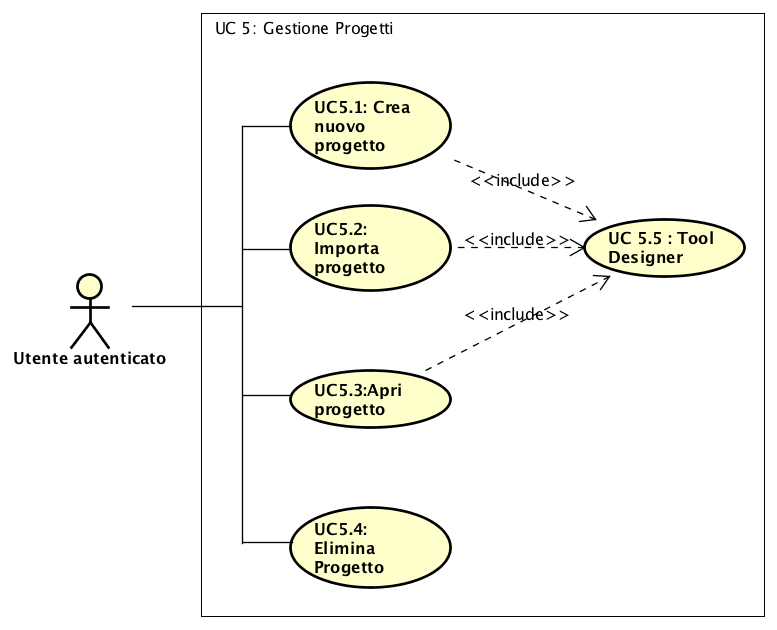
\includegraphics[scale=0.5]{../../Casi D'uso/UC5.png} 
\caption{Caso d'uso UC5} 
 \end{figure} 
\begin{itemize} 
\item \textbf{Attori}: Utente autenticato;
\item \textbf{Descrizione}: L’ attore ha la possibilità di aggiungere un nuovo progetto e di aprire o modificare un progetto già esistente;
\item \textbf{Precondizione}: L'applicazione è pronta e l'attore intende gestire un progetto;
\item \textbf{Postcondizione}: L’ applicazione visualizza la lista delle funzionalità disponibili;
\item \textbf{Scenario principale}: \begin{enumerate}\item Aggiunta Progetto (UC5.1);\item Apertura progetto (UC5.2);\item Eliminazione Progetto (UC5.3). 
 \end{enumerate}
\end{itemize} 
\newpage
\subsection{UC5.1 - Aggiunta Progetto} 
\label{ssec:UC5.1} 
\begin{figure}[h!] 
\centering 
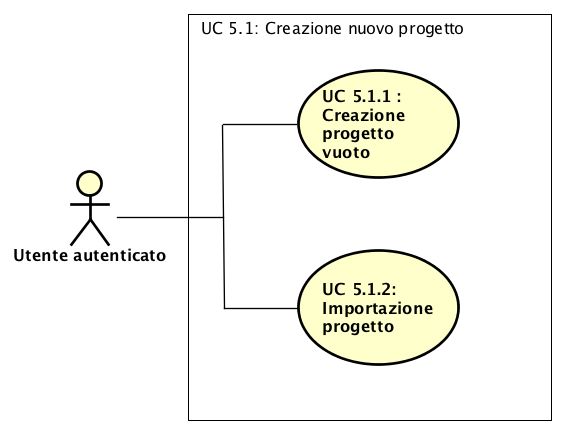
\includegraphics[scale=0.5]{../../Casi D'uso/UC5.1.png} 
\caption{Caso d'uso UC5.1} 
 \end{figure} 
\begin{itemize} 
\item \textbf{Attori}: Utente autenticato;
\item \textbf{Descrizione}: L’attore ha la possibilità di creare o importare un progetto;
\item \textbf{Precondizione}: L’attore vuole aggiungere un nuovo progetto alla lista;
\item \textbf{Postcondizione}: L’applicazione apre la lista dei modi per aggiungere un progetto;
\item \textbf{Scenario principale}: \begin{enumerate}\item Creazione Progetto vuoto (UC5.1.1);\item Importazione Progetto (UC5.1.2);
 \end{enumerate}
\item \textbf{Scenari alternativi}: L'attore decide di non aggiungere un nuovo progetto.
\end{itemize} 
\subsection{UC5.1.1 - Creazione Progetto vuoto} 
\label{ssec:UC5.1.1} 
\begin{itemize} 
\item \textbf{Attori}: Utente autenticato;
\item \textbf{Descrizione}: L'attore può creare un nuovo progetto;
\item \textbf{Precondizione}: L'attore vuole creare un progetto vuoto;
\item \textbf{Postcondizione}: L'applicazione crea un nuovo progetto vuoto;
\item \textbf{Scenari alternativi}: L'attore annulla la creazione del nuovo progetto.
\end{itemize} 
\newpage
\subsection{UC5.1.2 - Importazione Progetto} 
\label{ssec:UC5.1.2} 
\begin{itemize} 
\item \textbf{Attori}: Utente autenticato;
\item \textbf{Descrizione}: L'attore può importare un progetto;
\item \textbf{Precondizione}: L'attore vuole importare un progetto;
\item \textbf{Postcondizione}: L'applicazione importa il progetto richiesto;
\item \textbf{Scenari alternativi}: L'attore decide di non importare nessun progetto.
\end{itemize} 
\subsection{UC5.2 - Apertura progetto} 
\label{ssec:UC5.2} 
\begin{itemize} 
\item \textbf{Attori}: Utente autenticato.
\item \textbf{Descrizione}: L’attore ha la possibilità di aprire un progetto precedentemente salvato.;
\item \textbf{Precondizione}: L’applicazione rende disponibile la lista dei progetti dell'attore;
\item \textbf{Postcondizione}: L’applicazione apre il progetto selezionato.
\end{itemize} 
\subsection{UC5.3 - Eliminazione Progetto} 
\label{ssec:UC5.3} 
\begin{itemize} 
\item \textbf{Attori}: Utente autenticato;
\item \textbf{Descrizione}: L'attore ha la possibilità di eliminare un progetto precedentemente salvato;
\item \textbf{Precondizione}: L’applicazione rende disponibile la lista dei progetti salvati dall'attore;
\item \textbf{Postcondizione}: L’applicazione elimina il progetto selezionato.
\end{itemize} 
\newpage
\subsection{UC6 - Tool Designer} 
\label{ssec:UC6} 
\begin{figure}[h!] 
\centering 
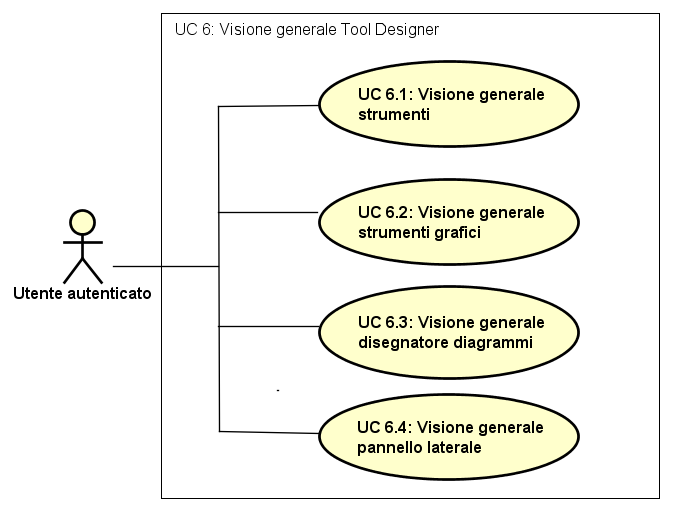
\includegraphics[scale=0.5]{../../Casi D'uso/UC6.png} 
\caption{Caso d'uso UC6} 
 \end{figure} 
\begin{itemize} 
\item \textbf{Attori}: Utente autenticato;
\item \textbf{Descrizione}: L'applicazione visualizza l'editor dei diagrammi;
\item \textbf{Precondizione}: L' attore ha effettuato l'accesso;
\item \textbf{Postcondizione}: L'applicazione visualizza la finestra;
\item \textbf{Scenario principale}: \begin{enumerate}\item Menù (UC6.1);\item Barra degli strumenti (UC6.2);\item Disegnatore diagrammi (UC6.3);\item Pannello laterale (UC6.4). 
 \end{enumerate}
\end{itemize} 
\newpage
\subsection{UC6.1 - Menù} 
\label{ssec:UC6.1} 
\begin{figure}[h!] 
\centering 
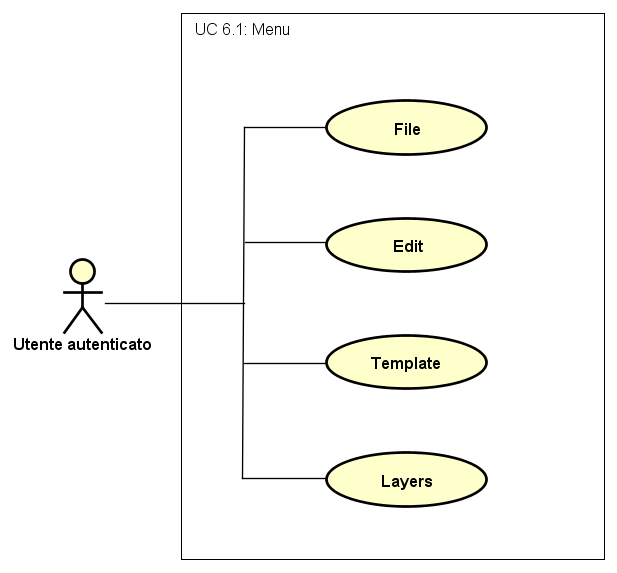
\includegraphics[scale=0.5]{../../Casi D'uso/UC6.1.png} 
\caption{Caso d'uso UC6.1} 
 \end{figure} 
\begin{itemize} 
\item \textbf{Attori}: Utente autenticato;
\item \textbf{Descrizione}: L’ attore può accedere alle voci file, edit, tool,
layers appartenenti al menù del Tool Designer;
\item \textbf{Precondizione}: L’applicazione offre all’utente una barra dei menù;
\item \textbf{Postcondizione}: L’applicazione, a seconda dell’operazione richiesta dall’utente,
svolge le sue funzioni;
\item \textbf{Scenario principale}: \begin{enumerate}\item File (UC6.1.1);\item Edit (UC6.1.2);\item Template (UC6.1.3);\item Layers (UC6.1.4). 
 \end{enumerate}
\end{itemize} 
\newpage
\subsection{UC6.1.1 - File} 
\label{ssec:UC6.1.1} 
\begin{figure}[h!] 
\centering 
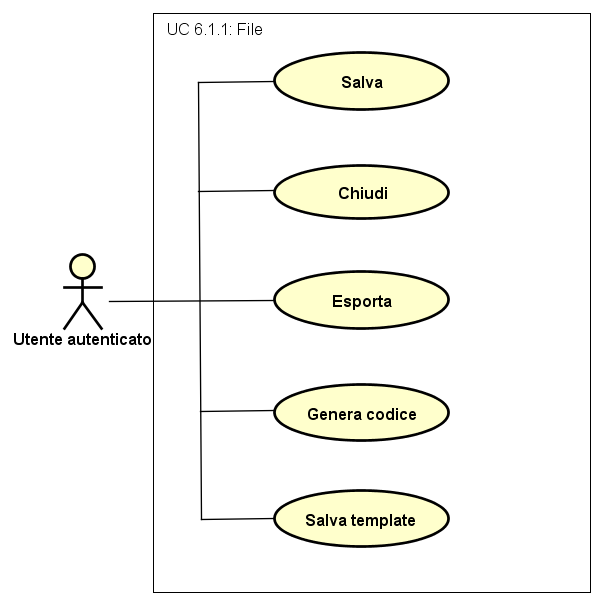
\includegraphics[scale=0.5]{../../Casi D'uso/UC6.1.1.png} 
\caption{Caso d'uso UC6.1.1} 
 \end{figure} 
\begin{itemize} 
\item \textbf{Attori}: Utente autenticato;
\item \textbf{Descrizione}: L’attore può accedere alle voci salva, chiudi, esporta, genera codice e salva template appartenenti alla voce file del menù;
\item \textbf{Precondizione}: L’applicazione offre all’attore la voce file nella barra dei menù;
\item \textbf{Postcondizione}: L’applicazione, a seconda dell’operazione richiesta dall’utente,
svolge le sue funzioni;
\item \textbf{Scenario principale}: \begin{enumerate}\item Salvataggio (UC6.1.1.1);\item Chiusura (UC6.1.1.2);\item Esportazione (UC6.1.1.3);\item Genera codice (UC6.1.1.4);\item Salvataggio template (UC6.1.1.5). 
 \end{enumerate}
\end{itemize} 
\newpage
\subsection{UC6.1.1.1 - Salvataggio} 
\label{ssec:UC6.1.1.1} 
\begin{itemize} 
\item \textbf{Attori}: Utente autenticato;
\item \textbf{Descrizione}: L’attore può salvare il suo progetto nello stato corrente;
\item \textbf{Precondizione}: L’attore ha aperto un progetto;
\item \textbf{Postcondizione}: L’applicazione salva il progetto nello stato corrente.
\end{itemize} 
\subsection{UC6.1.1.2 - Chiusura} 
\label{ssec:UC6.1.1.2} 
\begin{itemize} 
\item \textbf{Attori}: Utente autenticato;
\item \textbf{Descrizione}: L’attore può chiudere il progetto corrente;
\item \textbf{Precondizione}: L'attore ha aperto un progetto;
\item \textbf{Postcondizione}: L’applicazione chiude il progetto corrente.
\end{itemize} 
\subsection{UC6.1.1.3 - Esportazione} 
\label{ssec:UC6.1.1.3} 
\begin{itemize} 
\item \textbf{Attori}: Utente autenticato;
\item \textbf{Descrizione}: L’attore può esportare il progetto corrente per possederne una copia digitale;
\item \textbf{Precondizione}: L’attore ha un progetto aperto;
\item \textbf{Postcondizione}: L’applicazione esporta il progetto in un formato compresso.
\end{itemize} 
\subsection{UC6.1.1.4 - Genera codice} 
\label{ssec:UC6.1.1.4} 
\begin{itemize} 
\item \textbf{Attori}: Utente autenticato;
\item \textbf{Descrizione}: L’attore può generare il codice relativo all’UML prodotto;
\item \textbf{Precondizione}: L’attore vuole generare il codice dai suoi diagrammi UML;
\item \textbf{Postcondizione}: L’applicazione genera il codice relativo al disegno UML.
\end{itemize} 
\subsection{UC6.1.1.5 - Salvataggio template} 
\label{ssec:UC6.1.1.5} 
\begin{itemize} 
\item \textbf{Attori}: Utente autenticato;
\item \textbf{Descrizione}: L’attore ha la possibilità di salvare determinate classi o gerarchie, aggiungendole così alla lista di template già salvati;
\item \textbf{Precondizione}: L’applicazione offre all’attore la voce salva template, sottovoce di file nel menù, solamente se sono state create una o più classi, ed ognuna di esse ha un commento che le identifica;
\item \textbf{Postcondizione}: Viene aggiunto alla lista dei template il template desiderato.
\end{itemize} 
\newpage
\subsection{UC6.1.2 - Edit} 
\label{ssec:UC6.1.2} 
\begin{figure}[h!] 
\centering 
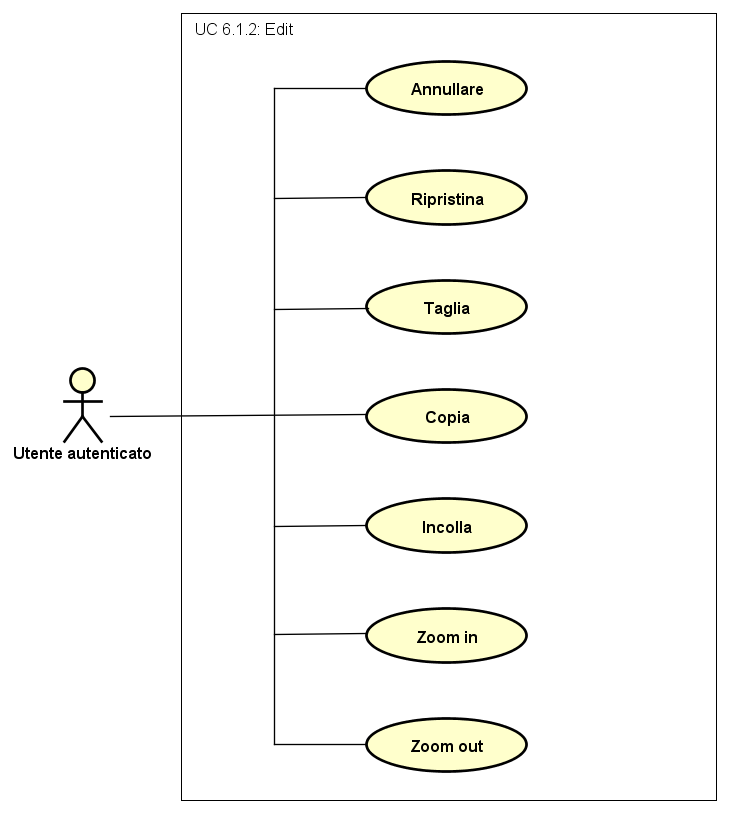
\includegraphics[scale=0.5]{../../Casi D'uso/UC6.1.2.png} 
\caption{Caso d'uso UC6.1.2} 
 \end{figure} 
\begin{itemize} 
\item \textbf{Attori}: Utente autenticato;
\item \textbf{Descrizione}: L’attore può accedere alle voci annulla, ripristina, taglia, copia, incolla, zoom in e zoom out appartenenti alla voce edit del menù;
\item \textbf{Precondizione}: L'attore ha aperto un progetto;
\item \textbf{Postcondizione}: L’applicazione visualizza la lista delle funzionalità disponibili;
\item \textbf{Scenario principale}: \begin{enumerate}\item Annulla (UC6.1.2.1);\item Ripristina (UC6.1.2.2);\item Taglia (UC6.1.2.3);\item Copia (UC6.1.2.4);\item Incolla (UC6.1.2.5);\item Zoom in (UC6.1.2.6);\item Zoom out (UC6.1.2.7). 
 \end{enumerate}
\end{itemize} 
\subsection{UC6.1.2.1 - Annulla} 
\label{ssec:UC6.1.2.1} 
\begin{itemize} 
\item \textbf{Attori}: Utente autenticato;
\item \textbf{Descrizione}: L’attore può tornare allo stato precedente l’ultima modifica;
\item \textbf{Precondizione}: L'attore ha un progetto aperto e ne ha effettuato una modifica;
\item \textbf{Postcondizione}: L’applicazione torna allo stato precedente l’ultima modifica.
\end{itemize} 
\subsection{UC6.1.2.2 - Ripristina} 
\label{ssec:UC6.1.2.2} 
\begin{itemize} 
\item \textbf{Attori}: Utente autenticato;
\item \textbf{Descrizione}: L’attore può ripristinare le modifiche effettuate successivamente allo stato attuale;
\item \textbf{Precondizione}: L’attore ha un progetto aperto ed ha annullato una modifica (UC 6.1.2.1);
\item \textbf{Postcondizione}: L’applicazione torna allo stato precedente l’ultima modifica.
\end{itemize} 
\subsection{UC6.1.2.3 - Taglia} 
\label{ssec:UC6.1.2.3} 
\begin{itemize} 
\item \textbf{Attori}: Utente autenticato;
\item \textbf{Descrizione}: L’attore può "tagliare" un determinato elemento del progetto;
\item \textbf{Precondizione}: L’attore ha un progetto aperto ed ha selezionato almeno un elemento dei diagrammi;
\item \textbf{Postcondizione}: L’applicazione taglia l’elemento selezionato.
\end{itemize} 
\subsection{UC6.1.2.4 - Copia} 
\label{ssec:UC6.1.2.4} 
\begin{itemize} 
\item \textbf{Attori}: Utente autenticato;
\item \textbf{Descrizione}: L’attore può "copiare" un determinato elemento del progetto.;
\item \textbf{Precondizione}: L’attore ha un progetto aperto ed ha selezionato almeno un elemento dei diagrammi;
\item \textbf{Postcondizione}: L’applicazione copia l’elemento selezionato.
\end{itemize} 
\subsection{UC6.1.2.5 - Incolla} 
\label{ssec:UC6.1.2.5} 
\begin{itemize} 
\item \textbf{Attori}: Utente autenticato;
\item \textbf{Descrizione}: L’attore può "incollare" un elemento precedentemente tagliato o copiato;
\item \textbf{Precondizione}: L’attore ha un progetto aperto ed ha selezionato almeno un elemento dei diagrammi;
\item \textbf{Postcondizione}: L’applicazione inserisce l’elemento designato.
\end{itemize} 
\subsection{UC6.1.2.6 - Zoom in} 
\label{ssec:UC6.1.2.6} 
\begin{itemize} 
\item \textbf{Attori}: Utente autenticato;
\item \textbf{Descrizione}: L’attore può ingrandire la visualizzazione di una determinata sezione;
\item \textbf{Precondizione}: L’attore ha un progetto aperto;
\item \textbf{Postcondizione}: L’applicazione ingrandisce gli elementi nella finestra del disegnatore dei diagrammi (UC 6.3).
\end{itemize} 
\subsection{UC6.1.2.7 - Zoom out} 
\label{ssec:UC6.1.2.7} 
\begin{itemize} 
\item \textbf{Attori}: Utente autenticato;
\item \textbf{Descrizione}: L’attore può rimpicciolire la visualizzazione di una determinata sezione;
\item \textbf{Precondizione}: L’attore ha un progetto aperto;
\item \textbf{Postcondizione}: L’applicazione rimpicciolisce gli elementi nella finestra del disegnatore dei diagrammi (UC 6.3).
\end{itemize} 
\newpage
\subsection{UC6.1.3 - Template} 
\label{ssec:UC6.1.3} 
\begin{figure}[h!] 
\centering 
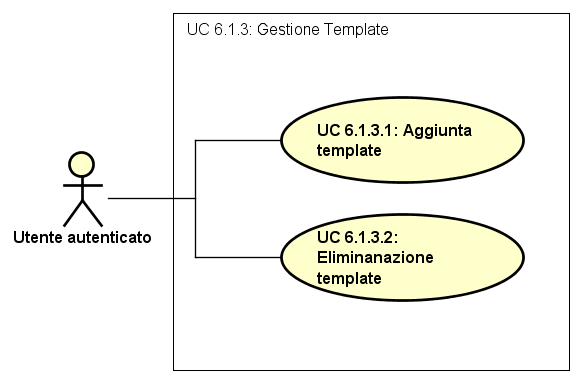
\includegraphics[scale=0.5]{../../Casi D'uso/UC6.1.3.png} 
\caption{Caso d'uso UC6.1.3} 
 \end{figure} 
\begin{itemize} 
\item \textbf{Attori}: Utente autenticato;
\item \textbf{Descrizione}: L’attore può accedere alla visualizzazione della lista dei template. I template visualizzati comprendono sia quelli già dati dagli sviluppatore, sia i propri template;
\item \textbf{Precondizione}: L’attore ha aperto un progetto;
\item \textbf{Postcondizione}: L'applicazione ha aperto una finestra dove viene visualizzata la lista dei template;
\item \textbf{Scenario principale}: \begin{enumerate}\item Aggiunta template (UC6.1.3.1);\item Eliminazione template (UC6.1.3.2). 
 \end{enumerate}
\end{itemize} 
\subsection{UC6.1.3.1 - Aggiunta template} 
\label{ssec:UC6.1.3.1} 
\begin{itemize} 
\item \textbf{Attori}: Utente autenticato;
\item \textbf{Descrizione}: L'attore può inserire nella finestra del disegnatore dei diagrammi (UC 6.3) il template selezionato;
\item \textbf{Precondizione}: L'attore ha aperto la finestra di gestione dei template;
\item \textbf{Postcondizione}: L'attore aggiunge il template selezionato nella finestra del disegnatore dei diagrammi(UC 6.3);
\item \textbf{Scenari alternativi}: L'attore chiude la finestra di gestione template (UC 6.1.3) e non viene effettuata nessuna operazione.
\end{itemize} 
\subsection{UC6.1.3.2 - Eliminazione template} 
\label{ssec:UC6.1.3.2} 
\begin{itemize} 
\item \textbf{Attori}: Utente autenticato;
\item \textbf{Descrizione}: L'attore può eliminare dalla lista il template selezionato;
\item \textbf{Precondizione}: L'attore ha aperto la finestra di gestione dei template (UC 6.1.3);
\item \textbf{Postcondizione}: Il template selezionato viene rimosso dalla lista;
\item \textbf{Scenari alternativi}: L'attore chiude la finestra di gestione template (UC 6.1.3) e non viene effettuata nessuna operazione.
\end{itemize} 
\newpage
\subsection{UC6.1.4 - Layers} 
\label{ssec:UC6.1.4} 
\begin{figure}[h!] 
\centering 
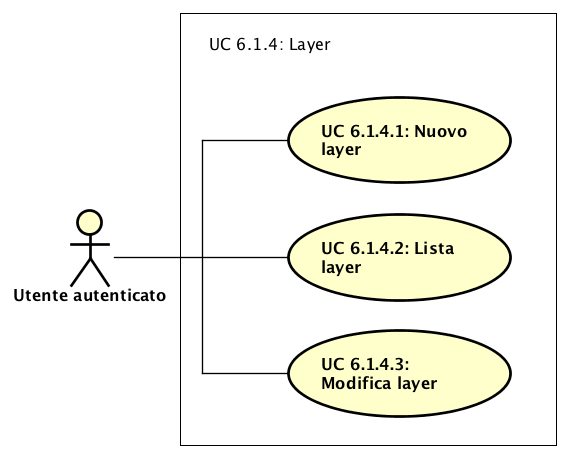
\includegraphics[scale=0.5]{../../Casi D'uso/UC6.1.4.png} 
\caption{Caso d'uso UC6.1.4} 
 \end{figure} 
\begin{itemize} 
\item \textbf{Attori}: Utente autenticato;
\item \textbf{Descrizione}: L’attore  può accedere alla visualizzazione della lista dei layers. Può inoltre creare nuovi layer oppure rinominarne o eliminarne di già esistenti;
\item \textbf{Precondizione}: L’attore ha un progetto aperto;
\item \textbf{Postcondizione}: L'applicazione visualizza la lista delle funzionalità disponibili sui layer;
\item \textbf{Scenario principale}: \begin{enumerate}\item Nuovo layer (UC6.1.4.1);\item Lista layer (UC6.1.4.2);\item Modifica layer (UC6.1.4.3). 
 \end{enumerate}
\end{itemize} 
\subsection{UC6.1.4.1 - Nuovo layer} 
\label{ssec:UC6.1.4.1} 
\begin{itemize} 
\item \textbf{Attori}: Utente autenticato;
\item \textbf{Descrizione}: L'attore crea un nuovo layer a cui è possibile assegnare delle classi;
\item \textbf{Precondizione}: L'attore ha aperto la finestra di gestione dei layer;
\item \textbf{Postcondizione}: L'attore ha aggiunto un nuovo layer assegnandogli il nome desiderato.
\end{itemize} 
\subsection{UC6.1.4.2 - Lista layer} 
\label{ssec:UC6.1.4.2} 
\begin{itemize} 
\item \textbf{Attori}: Utente autenticato;
\item \textbf{Descrizione}: L'attore seleziona il layer di cui desidera visualizzare le classi che gli sono state assegnate;
\item \textbf{Precondizione}: L'attore ha aperto la finestra di gestione dei layer;
\item \textbf{Postcondizione}: L'attore ha visualizzato le classi assegnate al layer desiderato.
\end{itemize} 
\newpage
\subsection{UC6.1.4.3 - Modifica layer} 
\label{ssec:UC6.1.4.3} 
\begin{figure}[h!] 
\centering 
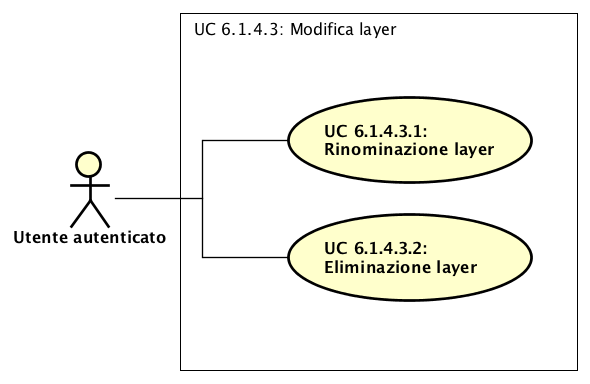
\includegraphics[scale=0.5]{../../Casi D'uso/UC6.1.4.3.png} 
\caption{Caso d'uso UC6.1.4.3} 
 \end{figure} 
\begin{itemize} 
\item \textbf{Attori}: Utente autenticato;
\item \textbf{Descrizione}: L'attore desidera rinominare oppure eliminare un layer tra quelli esistenti;
\item \textbf{Precondizione}: L'attore ha aperto la finestra di gestione dei layer;
\item \textbf{Postcondizione}: L'applicazione apre la finestra di gestione dei layer;
\item \textbf{Scenario principale}: \begin{enumerate}\item Rinominazione layer (UC6.1.4.3.1);\item Eliminazione layer (UC6.1.4.3.2). 
 \end{enumerate}
\end{itemize} 
\subsection{UC6.1.4.3.1 - Rinominazione layer} 
\label{ssec:UC6.1.4.3.1} 
\begin{itemize} 
\item \textbf{Attori}: Utente autenticato;
\item \textbf{Descrizione}: L'attore desidera rinominare un layer tra quelli esistenti;
\item \textbf{Precondizione}: L'attore seleziona il layer da rinominare;
\item \textbf{Postcondizione}: L'attore ha modificato il nome del layer che intendeva modificare, mantenendo tutte le classi associate.
\end{itemize} 
\subsection{UC6.1.4.3.2 - Eliminazione layer} 
\label{ssec:UC6.1.4.3.2} 
\begin{itemize} 
\item \textbf{Attori}: Utente autenticato;
\item \textbf{Descrizione}: L'attore desidera eliminare un layer tra quelli esistenti;
\item \textbf{Precondizione}: L'attore seleziona un layer;
\item \textbf{Postcondizione}: L'applicazione ha eliminato il layer che intendeva modificare e tutte le classi assegnate a tale layer, se ce n'erano, non risultano più assegnate a nessun layer.
\end{itemize} 
\newpage
\subsection{UC6.2 - Barra degli strumenti} 
\label{ssec:UC6.2} 
\begin{figure}[h!] 
\centering 
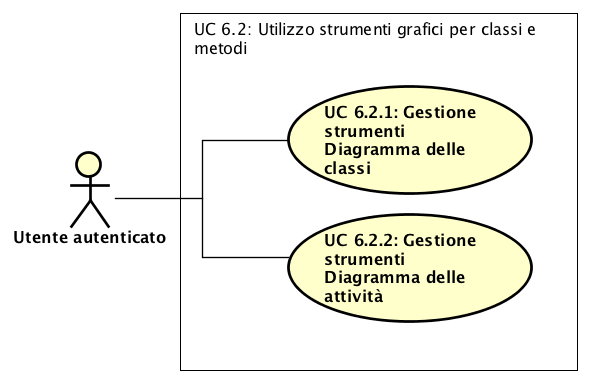
\includegraphics[scale=0.5]{../../Casi D'uso/UC6.2.png} 
\caption{Caso d'uso UC6.2} 
 \end{figure} 
\begin{itemize} 
\item \textbf{Attori}: Utente autenticato;
\item \textbf{Descrizione}: L'applicazione visualizza la barra degli strumenti grafici;
\item \textbf{Precondizione}: L'attore ha effettuato l'accesso;
\item \textbf{Postcondizione}: L'applicazione visualizza la barra degli strumenti grafici;
\item \textbf{Scenario principale}: \begin{enumerate}\item Strumenti delle classi (UC6.2.1);\item Strumenti Diagramma delle Attività (UC6.2.2). 
 \end{enumerate}
\end{itemize} 
\newpage
\subsection{UC6.2.1 - Strumenti delle classi} 
\label{ssec:UC6.2.1}
\begin{figure}[h!] 
\centering 
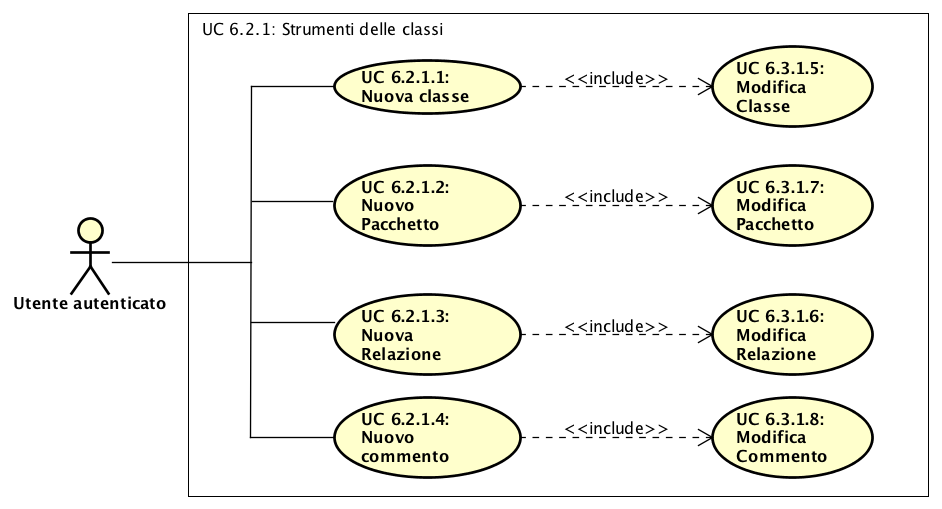
\includegraphics[scale=0.5]{../../Casi D'uso/UC6.2.1.png} 
\caption{Caso d'uso UC6.2.1} 
 \end{figure}  
\begin{itemize} 
\item \textbf{Attori}: Utente autenticato;
\item \textbf{Descrizione}: L'attore, per la creazione di un diagramma della classi ha la possibilità di selezionare una nuova classe, inserire un package per raggruppare delle classi o inserire delle relazioni tra le classi;
\item \textbf{Precondizione}: L'attore ha aperto un progetto;
\item \textbf{Postcondizione}: L'applicazione visualizza gli strumenti per disegnare le classi;
\item \textbf{Scenario principale}: \begin{enumerate}\item Nuova Classe (UC6.2.1.1);\item Nuovo Pacchetto (UC6.2.1.2);\item Nuova Relazione (UC6.2.1.3);\item Nuovo commento (UC6.2.1.4); 
 \end{enumerate}
 \item \textbf{Inclusioni}: \begin{itemize}
 	\item \textbf{ Modifica Classe (UC 6.3.1.5)};
 	\item \textbf{ Modifica Pacchetto (UC 6.3.1.7)};
 	\item \textbf{ Modifica Relazione (UC 6.3.1.6)};
 	\item \textbf{ Modifica Commento (UC 6.3.1.8)}.
 \end{itemize}
\end{itemize} 
\subsection{UC6.2.1.1 - Nuova Classe} 
\label{ssec:UC6.2.1.1} 
\begin{itemize} 
\item \textbf{Attori}: Utente autenticato:
\item \textbf{Descrizione}: L'attore ha la possibilità di inserire il disegno rappresentante una classe nello standard UML con i relativi campi compilati;
\item \textbf{Precondizione}: L'attore ha un progetto aperto;
\item \textbf{Postcondizione}: Viene rappresentato il disegno della classe e vengono salvati i dati contenuti in essa.
\end{itemize} 
\subsection{UC6.2.1.2 - Nuovo Pacchetto} 
\label{ssec:UC6.2.1.2} 
\begin{itemize} 
\item \textbf{Attori}: Utente autenticato;
\item \textbf{Descrizione}: L'attore ha la possibilità di inserire il disegno rappresentante un package nello standard UML;
\item \textbf{Precondizione}: L'attore ha un progetto aperto;
\item \textbf{Postcondizione}: L'applicazione rappresentata il disegno del package e vengono salvati i relativi dati.
\end{itemize} 
\newpage
\subsection{UC6.2.1.3 - Nuova Relazione} 
\label{ssec:UC6.2.1.3} 
\begin{figure}[h!] 
\centering 
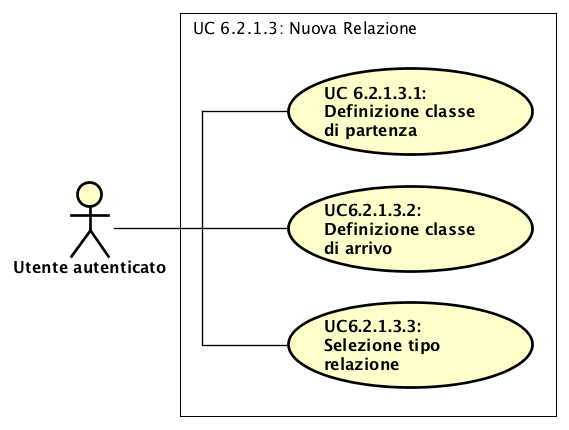
\includegraphics[scale=0.5]{../../Casi D'uso/UC6.2.1.3.png} 
\caption{Caso d'uso UC6.2.1.3} 
 \end{figure} 
\begin{itemize} 
\item \textbf{Attori}: Utente autenticato;
\item \textbf{Descrizione}: L'applicazione fornisce una lista di relazioni tra le classi;
\item \textbf{Precondizione}: L'attore ha aperto un progetto;
\item \textbf{Postcondizione}: L'applicazione fornisce una lista di relazioni tra le classi;
\item \textbf{Scenario principale}: \begin{enumerate}\item Definizione classe di partenza (UC6.2.1.3.1);\item Definizione classe di arrivo (UC6.2.1.3.2);\item Selezione tipo relazione (UC6.2.1.3.3). 
 \end{enumerate}
\end{itemize} 
\subsection{UC6.2.1.3.1 - Definizione classe di partenza} 
\label{ssec:UC6.2.1.3.1} 
\begin{itemize} 
\item \textbf{Attori}: Utente autenticato;
\item \textbf{Descrizione}: Viene definito il punto di partenza dell'associazione;
\item \textbf{Precondizione}: Esiste almeno una classe;
\item \textbf{Postcondizione}: L'applicazione associa il disegno dell'assegnazione alla relativa classe.
\end{itemize} 
\subsection{UC6.2.1.3.2 - Definizione classe di arrivo} 
\label{ssec:UC6.2.1.3.2} 
\begin{itemize} 
\item \textbf{Attori}: Utente autenticato;
\item \textbf{Descrizione}: Viene definito il punto di arrivo dell'associazione;
\item \textbf{Precondizione}: Esiste almeno una classe;
\item \textbf{Postcondizione}: L'applicazione associa il disegno dell'assegnazione alla relativa classe di destinazione.
\end{itemize} 
\subsection{UC6.2.1.3.3 - Selezione tipo relazione} 
\label{ssec:UC6.2.1.3.3} 
\begin{itemize} 
\item \textbf{Attori}: Utente autenticato;
\item \textbf{Descrizione}: L'attore seleziona il tipo di relazione tra: dipendenza, associazione, gerarchia;
\item \textbf{Precondizione}: L'applicazione visualizza il form per l'inserimento dei dati;
\item \textbf{Postcondizione}: L'applicazione ha registrato i dati inseriti.
\end{itemize} 
\subsection{UC6.2.1.4 - Nuovo commento} 
\label{ssec:UC6.2.1.4} 
\begin{itemize} 
\item \textbf{Attori}: Utente autenticato;
\item \textbf{Descrizione}: L'attore ha la possibilità di inserire un commento associato ad un elemento del diagramma delle classi;
\item \textbf{Precondizione}: L'attore ha aperto un progetto;
\item \textbf{Postcondizione}: L'applicazione rappresentata un rettangolo testuale con all'interno il testo inserito;
\item \textbf{Scenario principale}: \begin{enumerate}\item Aggiunta relazione commento (UC6.2.1.4.1). 
 \end{enumerate}
\end{itemize} 
\subsection{UC6.2.1.4.1 - Aggiunta relazione commento} 
\label{ssec:UC6.2.1.4.1} 
\begin{itemize} 
\item \textbf{Attori}: Utente autenticato;
\item \textbf{Descrizione}: Il commento può associato ad un qualsiasi elemento del diagramma delle classi;
\item \textbf{Precondizione}: È presente almeno un elemento;
\item \textbf{Postcondizione}: Il commento è stato associato ad un elemento.
\end{itemize} 
\subsection{UC6.2.2 - Strumenti Diagramma delle Attività} 
\label{ssec:UC6.2.2} 
\begin{figure}[H] 
\centering 
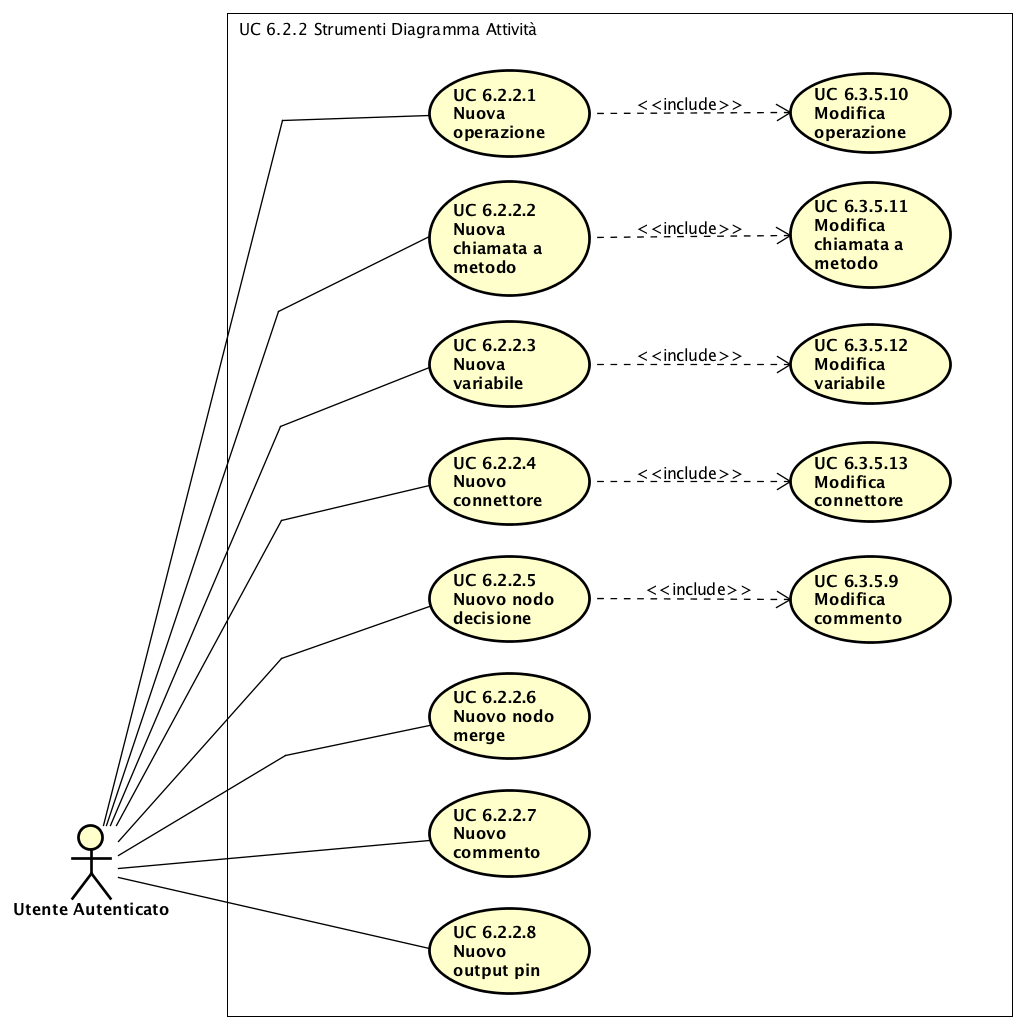
\includegraphics[scale=0.5]{../../Casi D'uso/UC6.2.2.png} 
\caption{Caso d'uso UC6.2.2} 
 \end{figure} 
\begin{itemize} 
\item \textbf{Attori}: Utente autenticato;
\item \textbf{Descrizione}: L'attore può selezionare da questa lista uno degli strumenti per la creazione di diagrammi delle attività;
\item \textbf{Precondizione}: L'attore deve aver caricato un progetto;
\item \textbf{Postcondizione}: L'applicazione visualizza la lista di strumenti necessari per il disegno di diagrammi delle attività;
\item \textbf{Scenario principale}: \begin{enumerate}\item Nuova operazione (UC6.2.2.1);\item Nuova chiamata a metodo (UC6.2.2.2);\item Nuova variabile (UC6.2.2.3);\item Nuovo connettore (UC6.2.2.4);\item Nuovo nodo decisione (UC6.2.2.5);\item Nuovo nodo merge (UC6.2.2.6);\item Nuovo commento (UC6.2.2.7);\item Nuovo output pin (UC6.2.2.8);
 \end{enumerate}
 \item \textbf{Inclusioni}: \begin{itemize}
 \item \textbf{ Modifica operazione (UC 6.3.5.10)};
 \item \textbf{ Modifica chiamata a metodo (UC 6.3.5.11)};
 \item \textbf{ Modifica variabile (UC 6.3.5.12)};
  \item \textbf{ Modifica connettore (UC 6.3.5.13)};
  \item \textbf{ Modifica commento (UC 6.3.5.9)};
 \end{itemize}
 
\end{itemize} 
\subsection{UC6.2.2.1 - Nuova operazione} 
\label{ssec:UC6.2.2.1} 
\begin{itemize} 
\item \textbf{Attori}: Utente autenticato;
\item \textbf{Descrizione}: L'attore può aggiungere un nuovo elemento operazione al diagramma delle attività di un metodo;
\item \textbf{Precondizione}: Viene selezionato un metodo di una classe che risiede nel frame del diagramma delle  classi;
\item \textbf{Postcondizione}: Viene aggiunto al diagramma delle attività di un metodo un nuovo elemento operazione;
\item \textbf{Scenari alternativi}: L'elemento non è posizionato all'interno della finestra del diagramma delle attività di un metodo.
\end{itemize} 
\subsection{UC6.2.2.2 - Nuova chiamata a metodo} 
\label{ssec:UC6.2.2.2} 
\begin{itemize} 
\item \textbf{Attori}: Utente autenticato;
\item \textbf{Descrizione}: L'attore può aggiungere un elemento "chiamata a metodo" al diagramma delle attività di un metodo;
\item \textbf{Precondizione}: Il metodo di una classe è stato selezionato ed è visualizzata correttamente la finestra del diagramma delle attività di esso;
\item \textbf{Postcondizione}: Un elemento chiamata a metodo è aggiunto al diagramma delle attività del metodo di una classe;
\item \textbf{Scenari alternativi}: L'elemento non è posizionato all'interno della finestra del diagramma delle attività di un metodo.
\end{itemize} 
\subsection{UC6.2.2.3 - Nuova variabile} 
\label{ssec:UC6.2.2.3} 
\begin{itemize} 
\item \textbf{Attori}: Utente autenticato;
\item \textbf{Descrizione}: L'attore può aggiungere un nuovo elemento variabile al diagramma delle attività di un metodo;
\item \textbf{Precondizione}: Viene selezionato un metodo di una classe che risiede nel frame del diagramma delle  classi;
\item \textbf{Postcondizione}: Viene aggiunto al diagramma delle attività di un metodo un nuovo elemento variabile.
\end{itemize} 
\subsection{UC6.2.2.4 - Nuovo connettore} 
\label{ssec:UC6.2.2.4} 
\begin{itemize} 
\item \textbf{Attori}: Utente autenticato;
\item \textbf{Descrizione}: L'attore può aggiungere un nuovo elemento connettore al diagramma delle attività di un metodo;
\item \textbf{Precondizione}: Viene selezionato un metodo di una classe che risiede nel frame del diagramma delle  classi; Devono esserci nel diagramma delle attività del metodo almeno due elementi che possono essere connessi;
\item \textbf{Postcondizione}: Viene aggiunto al diagramma delle attività di un metodo un nuovo elemento connettore;
\item \textbf{Scenari alternativi}: L'elemento non è posizionato all'interno della finestra del diagramma delle attività di un metodo.
\end{itemize} 
\subsection{UC6.2.2.5 - Nuovo nodo decisione} 
\label{ssec:UC6.2.2.5} 
\begin{itemize} 
\item \textbf{Attori}: Utente autenticato;
\item \textbf{Descrizione}: L'attore può aggiungere un nuovo elemento nodo decisione al diagramma delle attività di un metodo;
\item \textbf{Precondizione}: Viene selezionato un metodo di una classe che risiede nel frame del diagramma delle  classi;
\item \textbf{Postcondizione}: Viene aggiunto al diagramma delle attività di un metodo un nuovo elemento nodo decisione.
\end{itemize} 
\subsection{UC6.2.2.6 - Nuovo nodo merge} 
\label{ssec:UC6.2.2.6} 
\begin{itemize} 
\item \textbf{Attori}: Utente autenticato;
\item \textbf{Descrizione}: L'attore può aggiungere un nuovo elemento nodo merge al diagramma delle attività di un metodo;
\item \textbf{Precondizione}: Viene selezionato un metodo di una classe che risiede nel frame del diagramma delle  classi;
\item \textbf{Postcondizione}: Viene aggiunto al diagramma delle attività di un metodo un nuovo elemento nodo merge.
\end{itemize} 
\subsection{UC6.2.2.7 - Nuovo commento} 
\label{ssec:UC6.2.2.7} 
\begin{itemize} 
\item \textbf{Attori}: Utente autenticato;
\item \textbf{Descrizione}: L'attore può aggiungere un nuovo elemento commento al diagramma delle attività di un metodo;
\item \textbf{Precondizione}: Viene selezionato un metodo di una classe che risiede nel frame del diagramma delle  classi;
\item \textbf{Postcondizione}: Viene aggiunto al diagramma delle attività di un metodo un nuovo elemento commento.
\end{itemize} 
\subsection{UC6.2.2.8 - Nuovo output pin} 
\label{ssec:UC6.2.2.8} 
\begin{itemize} 
\item \textbf{Attori}: Utente autenticato;
\item \textbf{Descrizione}: L'attore può annettere un nuovo output pin ad un elemento chiamata a metodo, presente nel diagramma delle attività di un metodo;
\item \textbf{Precondizione}: Viene selezionato un metodo di una classe che risiede nel frame del diagramma delle  classi; è presente un elemento chiamata a metodo nel diagramma;
\item \textbf{Postcondizione}: Viene annesso ad un elemento chiamata a metodo, presente nel diagramma delle attività di un metodo, un nuovo elemento output pin.
\end{itemize} 
\newpage
\subsection{UC6.3 - Disegnatore diagrammi} 
\label{ssec:UC6.3} 
\begin{figure}[h!] 
\centering 
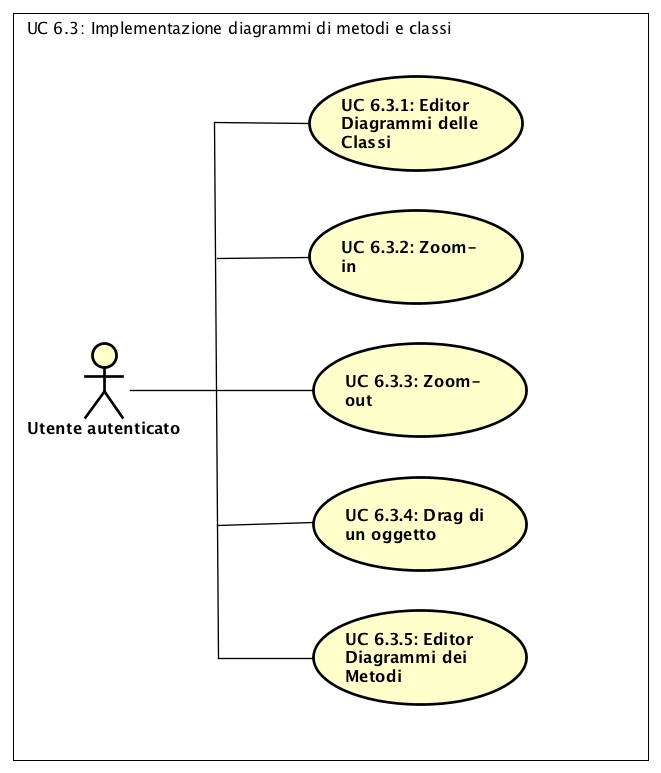
\includegraphics[scale=0.5]{../../Casi D'uso/UC6.3.png} 
\caption{Caso d'uso UC6.3} 
 \end{figure} 
\begin{itemize} 
\item \textbf{Attori}: Utente autenticato;
\item \textbf{Descrizione}: L'attore può implementare programmi disegnando diagrammi;
\item \textbf{Precondizione}: L'applicazione rende disponibile il frame di disegno;
\item \textbf{Postcondizione}: L'applicazione disegna i diagrammi richiesti dall'attore;
\item \textbf{Scenario principale}: \begin{enumerate}\item Editor Diagrammi delle Classi (UC6.3.1);\item Zoom-in (UC6.3.2);\item Zoom-out (UC6.3.3);\item Drag di un oggetto (UC6.3.4);\item Editor Diagrammi dei Metodi (UC6.3.5). 
 \end{enumerate}
\end{itemize} 
\newpage
\subsection{UC6.3.1 - Editor Diagrammi delle Classi} 
\label{ssec:UC6.3.1} 
\begin{figure}[h!] 
\centering 
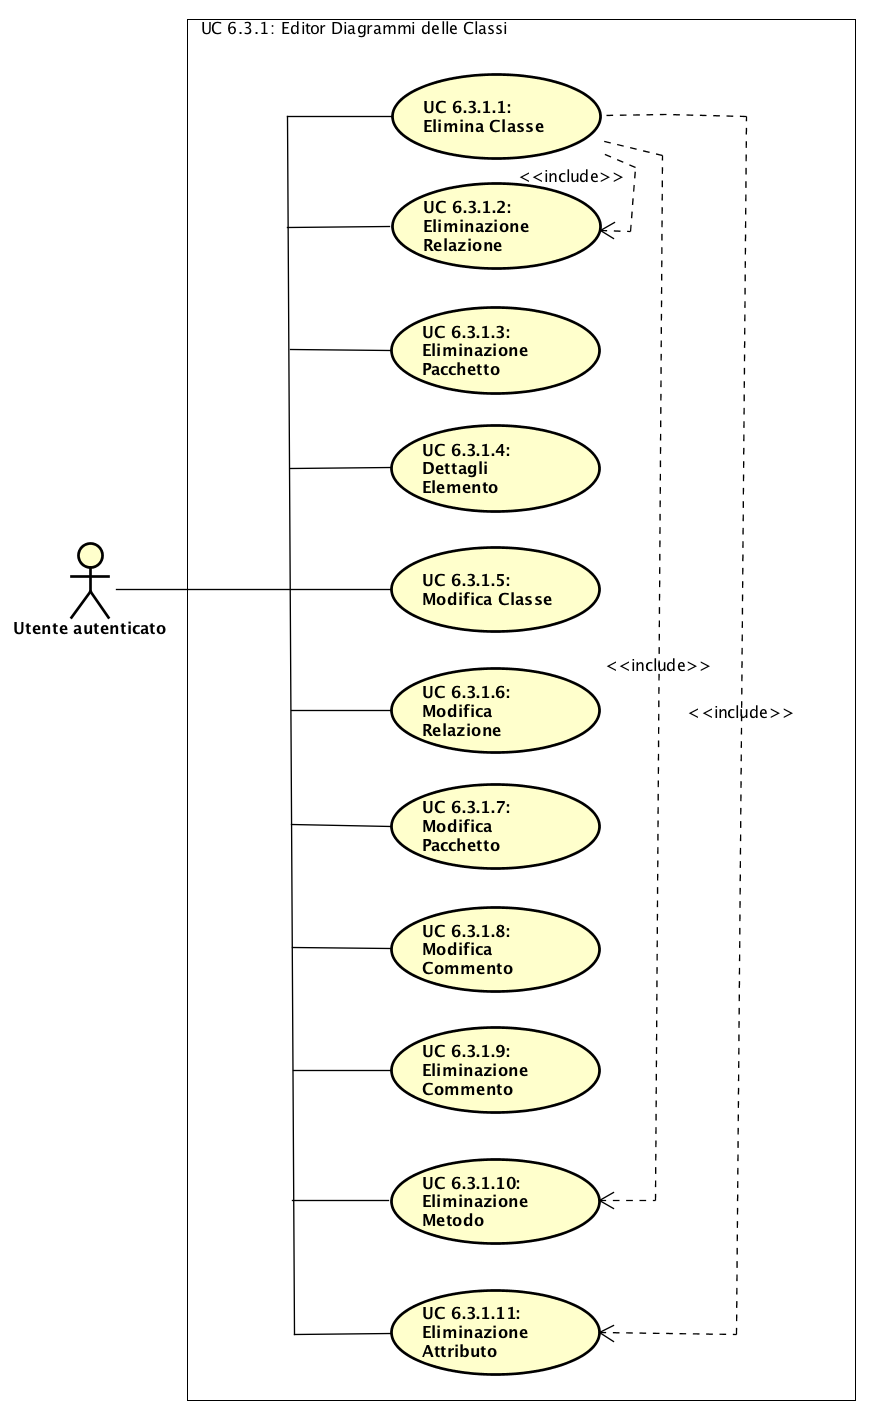
\includegraphics[scale=0.5]{../../Casi D'uso/UC6.3.1.png} 
\caption{Caso d'uso UC6.3.1} 
 \end{figure} 
\begin{itemize} 
\item \textbf{Attori}: Utente autenticato;
\item \textbf{Descrizione}: L'attore può interagire con la schermata principale;
\item \textbf{Precondizione}: L'attore crea o apre un progetto;
\item \textbf{Postcondizione}: L'attore chiude il progetto;
\item \textbf{Scenario principale}: \begin{enumerate}\item Eliminazione Classe (UC6.3.1.1);\item Eliminazione Relazione (UC6.3.1.2);\item Eliminazione pacchetto (UC6.3.1.3);\item Dettagli Elemento (UC6.3.1.4);\item Modifica Classe (UC6.3.1.5);\item Modifica Relazione (UC6.3.1.6);\item Modifica pacchetto (UC6.3.1.7);\item Modifica commento (UC6.3.1.8);\item Eliminazione commento (UC6.3.1.9). 
 \end{enumerate}
\end{itemize} 
\subsection{UC6.3.1.1 - Eliminazione Classe} 
\label{ssec:UC6.3.1.1} 
\begin{figure}[h!] 
\centering 
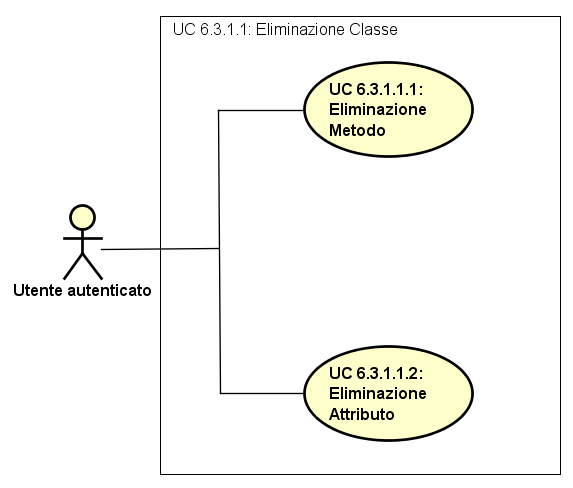
\includegraphics[scale=0.5]{../../Casi D'uso/UC6.3.1.1.png} 
\caption{Caso d'uso UC6.3.1.1} 
 \end{figure} 
\begin{itemize} 
\item \textbf{Attori}: Utente autenticato;
\item \textbf{Descrizione}: L'attore può eliminare una classe dal progetto corrente;
\item \textbf{Precondizione}: Deve essere stata disegnata una classe;
\item \textbf{Postcondizione}: Viene eliminata la classe selezionata e, a cascata, tutti i metodi ad essa, e solo ad essa, associati, tutti gli attributi e tutte le relazioni che la coinvolgono;
\item \textbf{Scenario principale}: \begin{enumerate}\item Eliminazione Metodo (UC6.3.1.1.1);\item Eliminazione Attributo (UC6.3.1.1.2). 
 \end{enumerate}
\end{itemize} 
\subsection{UC6.3.1.1.1 - Eliminazione Metodo} 
\label{ssec:UC6.3.1.1.1} 
\begin{itemize} 
\item \textbf{Attori}: Utente autenticato;
\item \textbf{Descrizione}: L'attore ha disegnato una classe con almeno un metodo ed  eventualmente anche il diagramma delle attività corrispondente e può eliminarlo;
\item \textbf{Precondizione}: È stata creata una classe con almeno un metodo;
\item \textbf{Postcondizione}: Viene eliminato il metodo selezionato e, a cascata, il diagramma delle attività associato se esistente;
\item \textbf{Scenari alternativi}: L'attore ha aggiunto un nuovo metodo e desidera eliminarlo.
\end{itemize} 
\subsection{UC6.3.1.1.2 - Eliminazione Attributo} 
\label{ssec:UC6.3.1.1.2} 
\begin{itemize} 
\item \textbf{Attori}: Utente autenticato;
\item \textbf{Descrizione}: L'attore ha disegnato una classe con almeno un attributo al suo interno e può eliminarlo;
\item \textbf{Precondizione}: È stata creata una classe con almeno un attributo;
\item \textbf{Postcondizione}: L'attributo selezionato viene eliminato;
\item \textbf{Scenari alternativi}: L'attore ha aggiunto un nuovo attributo e desidera eliminarlo.
\end{itemize} 
\subsection{UC6.3.1.2 - Eliminazione Relazione} 
\label{ssec:UC6.3.1.2} 
\begin{itemize} 
\item \textbf{Attori}: Utente autenticato;
\item \textbf{Descrizione}: L'attore può eliminare una relazione fra oggetti all'interno del designer;
\item \textbf{Precondizione}: È stata disegnata una relazione;
\item \textbf{Postcondizione}: Viene eliminata la relazione selezionata ed eventuali etichette associate.
\end{itemize} 
\subsection{UC6.3.1.3 - Eliminazione pacchetto} 
\label{ssec:UC6.3.1.3} 
\begin{itemize} 
\item \textbf{Attori}: Utente autenticato;
\item \textbf{Descrizione}: L'attore può eliminare un pacchetto;
\item \textbf{Precondizione}: È stato disegnato un pacchetto;
\item \textbf{Postcondizione}: Viene eliminato il pacchetto dal designer assieme a tutti i suoi eventuali elementi contenuti.
\end{itemize} 
\subsection{UC6.3.1.4 - Dettagli Elemento} 
\label{ssec:UC6.3.1.4} 
\begin{itemize} 
\item \textbf{Attori}: Utente autenticato;
\item \textbf{Descrizione}: L'attore può visualizzare i dettagli implementativi dell'elemento desiderato;
\item \textbf{Precondizione}: È stato disegnato almeno un elemento all'interno del designer;
\item \textbf{Postcondizione}: Vengono visualizzati tutti i dettagli dell'elemento.
\end{itemize} 
\newpage
\subsection{UC6.3.1.5 - Modifica Classe} 
\label{ssec:UC6.3.1.5} 
\begin{figure}[h!] 
\centering 
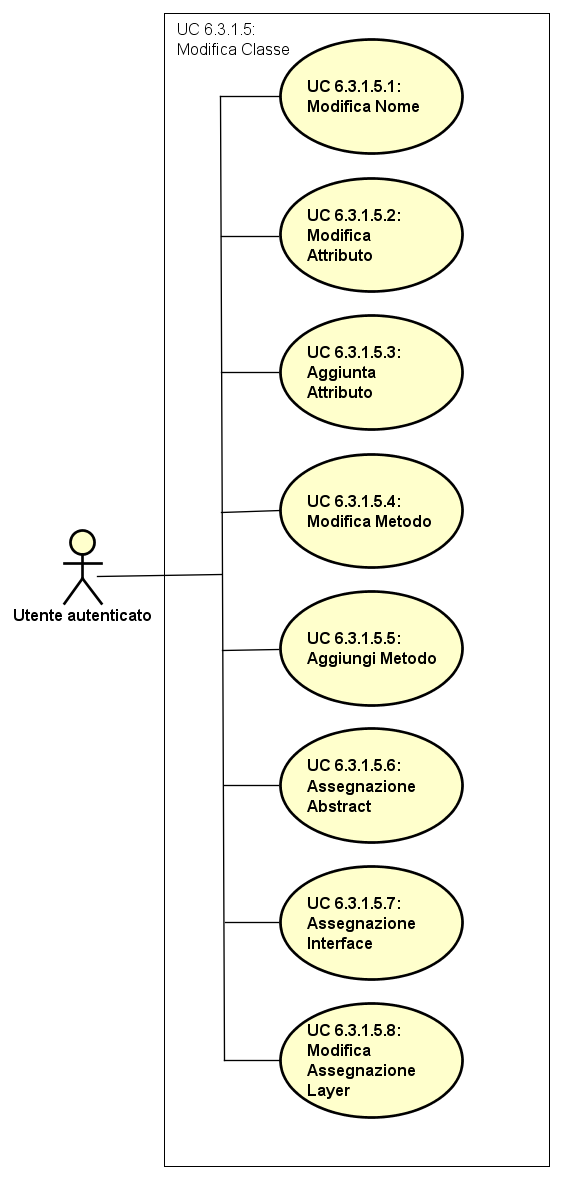
\includegraphics[scale=0.5]{../../Casi D'uso/UC6.3.1.5.png} 
\caption{Caso d'uso UC6.3.1.5} 
 \end{figure} 
\begin{itemize} 
\item \textbf{Attori}: Utente autenticato;
\item \textbf{Descrizione}: L'attore può modificare degli elementi interni ad una classe;
\item \textbf{Precondizione}: È stata disegnata una classe sul progetto;
\item \textbf{Postcondizione}: La classe risulta modificata;
\item \textbf{Scenario principale}: \begin{enumerate}\item Modifica Nome (UC6.3.1.5.1);\item Modifica Attributo (UC6.3.1.5.2);\item Aggiunta attributo (UC6.3.1.5.3);\item Modifica Metodo (UC6.3.1.5.4);\item Aggiungi Metodo (UC6.3.1.5.5);\item Assegnazione Abstract (UC6.3.1.5.6);\item Assegnazione interface (UC6.3.1.5.7);\item Modifica assegnazione layer (UC6.3.1.5.8). 
 \end{enumerate}
\end{itemize} 
\subsection{UC6.3.1.5.1 - Modifica Nome} 
\label{ssec:UC6.3.1.5.1} 
\begin{itemize} 
\item \textbf{Attori}: Utente autenticato;
\item \textbf{Descrizione}: L'attore può modificare il nome della classe;
\item \textbf{Precondizione}: È stata creata una classe con un nome;
\item \textbf{Postcondizione}: Viene modificato il nome della classe.
\end{itemize} 
\subsection{UC6.3.1.5.2 - Modifica Attributo} 
\label{ssec:UC6.3.1.5.2} 
\begin{figure}[h!] 
\centering 
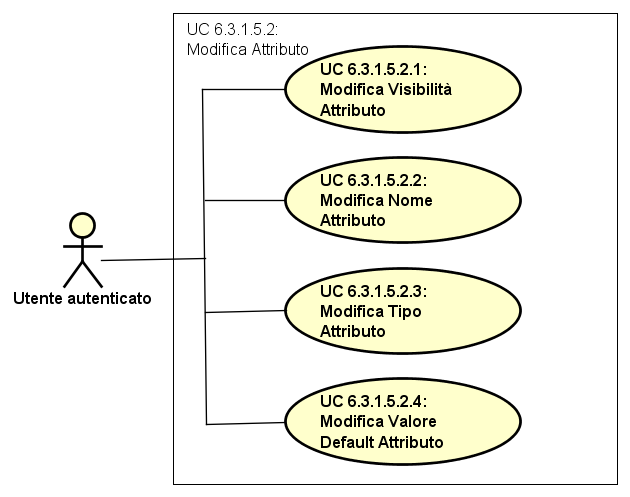
\includegraphics[scale=0.5]{../../Casi D'uso/UC6.3.1.5.2.png} 
\caption{Caso d'uso UC6.3.1.5.2} 
 \end{figure} 
\begin{itemize} 
\item \textbf{Attori}: Utente autenticato;
\item \textbf{Descrizione}: L'attore può modificare l'attributo della classe;
\item \textbf{Precondizione}: È stata disegnata una classe con almeno un attributo;
\item \textbf{Postcondizione}: Viene modificato l'attributo selezionato;
\item \textbf{Scenario principale}: \begin{enumerate}\item Modifica visibilità attributo (UC6.3.1.5.2.1);\item Modifica nome attributo (UC6.3.1.5.2.2);\item Modifica tipo attributo (UC6.3.1.5.2.3);\item Modifica valore default attributo (UC6.3.1.5.2.4). 
 \end{enumerate}
\end{itemize} 
\subsection{UC6.3.1.5.2.1 - Modifica visibilità attributo} 
\label{ssec:UC6.3.1.5.2.1} 
\begin{itemize} 
\item \textbf{Attori}: Utente autenticato;
\item \textbf{Descrizione}: L'attore può scegliere la visibilità per l'attributo;
\item \textbf{Precondizione}: Viene visualizzato un form che permette la selezione della visibilità;
\item \textbf{Postcondizione}: L'applicazione registra il dato inserito.
\end{itemize} 
\subsection{UC6.3.1.5.2.2 - Modifica nome attributo} 
\label{ssec:UC6.3.1.5.2.2} 
\begin{itemize} 
\item \textbf{Attori}: Utente autenticato;
\item \textbf{Descrizione}: L'attore può inserire il nome per l'attributo;
\item \textbf{Precondizione}: Viene visualizzato un form che permette l'inserimento del nome dell'attributo;
\item \textbf{Postcondizione}: L'applicazione registra il dato inserito.
\end{itemize} 
\subsection{UC6.3.1.5.2.3 - Modifica tipo attributo} 
\label{ssec:UC6.3.1.5.2.3} 
\begin{itemize} 
\item \textbf{Attori}: Utente autenticato;
\item \textbf{Descrizione}: L'attore può inserire il tipo dell'attributo che si sta inserendo;
\item \textbf{Precondizione}: Viene visualizzato un form che permette l'inserimento tipo dell'attributo;
\item \textbf{Postcondizione}: L'applicazione registra il dato inserito.
\end{itemize} 
\subsection{UC6.3.1.5.2.4 - Modifica valore default attributo} 
\label{ssec:UC6.3.1.5.2.4} 
\begin{itemize} 
\item \textbf{Attori}: Utente autenticato;
\item \textbf{Descrizione}: L'attore può inserire il valore di default che può avere l'attributo;
\item \textbf{Precondizione}: Viene visualizzato un form che permette l'inserimento del valore di default dell'attributo;
\item \textbf{Postcondizione}: L'applicazione registra il dato inserito.
\end{itemize} 
\subsection{UC6.3.1.5.3 - Aggiunta attributo} 
\label{ssec:UC6.3.1.5.3} 
\begin{itemize} 
\item \textbf{Attori}: Utente autenticato;
\item \textbf{Descrizione}: L'attore può inserire un attributo per la classe selezionata;
\item \textbf{Precondizione}: Viene visualizzato un form che permette l'inserimento di attributi della classe;
\item \textbf{Postcondizione}: L'applicazione registra il dato inserito.
\end{itemize} 
\subsection{UC6.3.1.5.4 - Modifica Metodo} 
\label{ssec:UC6.3.1.5.4} 
\begin{figure}[h!] 
\centering 
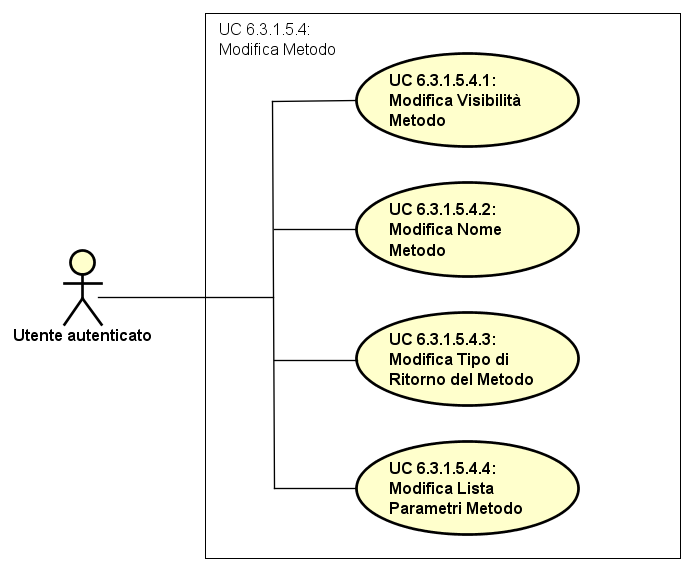
\includegraphics[scale=0.5]{../../Casi D'uso/UC6.3.1.5.4.png} 
\caption{Caso d'uso UC6.3.1.5.4} 
 \end{figure} 
\begin{itemize} 
\item \textbf{Attori}: Utente autenticato;
\item \textbf{Descrizione}: L'attore può modificare il metodo della classe;
\item \textbf{Precondizione}: È stata creata una classe con almeno un metodo al suo interno;
\item \textbf{Postcondizione}: Il metodo selezionato viene modificato;
\item \textbf{Scenario principale}: \begin{enumerate}\item Modifica visibilità metodo (UC6.3.1.5.4.1);\item Modifica nome metodo (UC6.3.1.5.4.2);\item Modifica tipo di ritorno del metodo (UC6.3.1.5.4.3);\item Modifica lista parametri metodo (UC6.3.1.5.4.4). 
 \end{enumerate}
\end{itemize} 
\subsection{UC6.3.1.5.4.1 - Modifica visibilità metodo} 
\label{ssec:UC6.3.1.5.4.1} 
\begin{itemize} 
\item \textbf{Attori}: Utente autenticato;
\item \textbf{Descrizione}: L'attore può scegliere la visibilità per un metodo;
\item \textbf{Precondizione}: Viene visualizzato un form che permette la selezione della visibilità;
\item \textbf{Postcondizione}: L'applicazione registra il dato inserito.
\end{itemize} 
\subsection{UC6.3.1.5.4.2 - Modifica nome metodo} 
\label{ssec:UC6.3.1.5.4.2} 
\begin{itemize} 
\item \textbf{Attori}: Utente autenticato;
\item \textbf{Descrizione}: L'attore può inserire il nome per il metodo;
\item \textbf{Precondizione}: Viene visualizzato un form che permette l'inserimento del nome del metodo;
\item \textbf{Postcondizione}: L'applicazione registra il dato inserito.
\end{itemize} 
\subsection{UC6.3.1.5.4.3 - Modifica tipo di ritorno del metodo} 
\label{ssec:UC6.3.1.5.4.3} 
\begin{itemize} 
\item \textbf{Attori}: Utente autenticato;
\item \textbf{Descrizione}: L'attore può inserire il tipo di ritorno per il metodo;
\item \textbf{Precondizione}: Viene visualizzato un form che permette l'inserimento tipo di ritorno del metodo;
\item \textbf{Postcondizione}: L'applicazione registra il dato inserito.
\end{itemize} 
\subsection{UC6.3.1.5.4.4 - Modifica lista parametri metodo} 
\label{ssec:UC6.3.1.5.4.4} 
\begin{itemize} 
\item \textbf{Attori}: Utente autenticato;
\item \textbf{Descrizione}: L'attore può inserire la lista dei parametri che verranno utilizzati nella realizzazione del metodo;
\item \textbf{Precondizione}: Viene visualizzato un form che permette l'inserimento della lista dei parametri;
\item \textbf{Postcondizione}: L'applicazione registra il dato inserito.
\end{itemize} 
\subsection{UC6.3.1.5.5 - Aggiungi Metodo} 
\label{ssec:UC6.3.1.5.5} 
\begin{itemize} 
\item \textbf{Attori}: Utente autenticato;
\item \textbf{Descrizione}: L'attore può aggiungere un metodo;
\item \textbf{Precondizione}: Deve essere presente la classe alla quale si vuole aggiungere il metodo;
\item \textbf{Postcondizione}: Il metodo viene aggiunto alla classe prescelta.
\end{itemize} 
\subsection{UC6.3.1.5.6 - Assegnazione Abstract} 
\label{ssec:UC6.3.1.5.6} 
\begin{itemize} 
\item \textbf{Attori}: Utente autenticato;
\item \textbf{Descrizione}: L'attore definisce se la classe è astratta;
\item \textbf{Precondizione}: Viene visualizzato un form che permette l'assegnazione della keyword <<abstract>>;
\item \textbf{Postcondizione}: L'applicazione registra il dato inserito.
\end{itemize} 
\subsection{UC6.3.1.5.7 - Assegnazione interface} 
\label{ssec:UC6.3.1.5.7} 
\begin{itemize} 
\item \textbf{Attori}: Utente autenticato;
\item \textbf{Descrizione}: L'attore definisce se la classe un'interfaccia;
\item \textbf{Precondizione}: Viene visualizzato un form che permette l'assegnazione della keyword <<interface>>;
\item \textbf{Postcondizione}: L'applicazione registra il dato inserito.
\end{itemize} 
\subsection{UC6.3.1.5.8 - Modifica assegnazione layer} 
\label{ssec:UC6.3.1.5.8} 
\begin{itemize} 
\item \textbf{Attori}: Utente autenticato;
\item \textbf{Descrizione}: L'attore può selezionare il layer a cui vuole associare la classe;
\item \textbf{Precondizione}: Viene visualizzato un form che permette l'assegnazione del layer;
\item \textbf{Postcondizione}: L'applicazione registra il dato inserito.
\end{itemize} 
\subsection{UC6.3.1.6 - Modifica Relazione} 
\label{ssec:UC6.3.1.6} 
\begin{itemize} 
\item \textbf{Attori}: Utente autenticato;
\item \textbf{Descrizione}: L'attore può modificare l'etichetta della relazione;
\item \textbf{Precondizione}: È stata creata una relazione fra due o più classi;
\item \textbf{Postcondizione}: L'etichetta della relazione corrente è stata modificata.
\end{itemize} 
\subsection{UC6.3.1.7 - Modifica pacchetto} 
\label{ssec:UC6.3.1.7} 
\begin{figure}[h!] 
\centering 
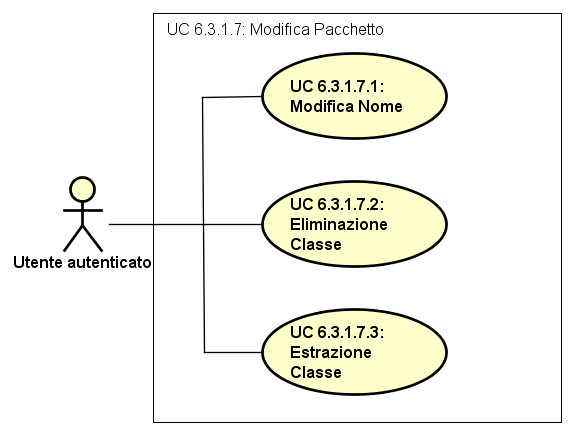
\includegraphics[scale=0.5]{../../Casi D'uso/UC6.3.1.7.png} 
\caption{Caso d'uso UC6.3.1.7} 
 \end{figure} 
\begin{itemize} 
\item \textbf{Attori}: Utente autenticato;
\item \textbf{Descrizione}: L'attore può modificare un pacchetto;
\item \textbf{Precondizione}: È stato creato un pacchetto;
\item \textbf{Postcondizione}: Il pacchetto è stato modificato;
\item \textbf{Scenario principale}: \begin{enumerate}\item Modifica Nome (UC6.3.1.7.1);\item Eliminazione classe (UC6.3.1.7.2);\item Estrazione classe (UC6.3.1.7.3). 
 \end{enumerate}
\end{itemize} 
\subsection{UC6.3.1.7.1 - Modifica Nome} 
\label{ssec:UC6.3.1.7.1} 
\begin{itemize} 
\item \textbf{Attori}: Utente autenticato.
\item \textbf{Descrizione}: L'attore può modificare il nome di un pacchetto, tale nome deve essere univoco;
\item \textbf{Precondizione}: È stato creato un pacchetto e viene visualizzato un form che permette l'inserimento del nome;
\item \textbf{Postcondizione}: Il nome del pacchetto selezionato viene salvato.
\end{itemize} 
\subsection{UC6.3.1.7.2 - Eliminazione classe} 
\label{ssec:UC6.3.1.7.2} 
\begin{itemize} 
\item \textbf{Attori}: Utente autenticato;
\item \textbf{Descrizione}: L'attore può eliminare una classe all'interno del pacchetto;
\item \textbf{Precondizione}: Esiste un pacchetto con almeno una classe al suo interno;
\item \textbf{Postcondizione}: La classe selezionata viene eliminata dal pacchetto.
\end{itemize} 
\subsection{UC6.3.1.7.3 - Estrazione classe} 
\label{ssec:UC6.3.1.7.3} 
\begin{itemize} 
\item \textbf{Attori}: Utente autenticato;
\item \textbf{Descrizione}: L'attore può estrarre una classe dal pacchetto;
\item \textbf{Precondizione}: Esiste un pacchetto con almeno una classe al suo interno;
\item \textbf{Postcondizione}: La classe selezionata si trova fuori dal pacchetto.
\end{itemize} 
\subsection{UC6.3.1.8 - Modifica commento} 
\label{ssec:UC6.3.1.8} 
\begin{itemize} 
\item \textbf{Attori}: Utente autenticato;
\item \textbf{Descrizione}: L'attore può modificare il testo inserito nel commento;
\item \textbf{Precondizione}: E' stato inserito un commento;
\item \textbf{Postcondizione}: Il commento risulta modificato;
\item \textbf{Scenario principale}: \begin{enumerate}\item Modifica testo commento (UC6.3.1.8.1). 
 \end{enumerate}
\end{itemize} 
\subsection{UC6.3.1.8.1 - Modifica testo commento} 
\label{ssec:UC6.3.1.8.1} 
\begin{itemize} 
\item \textbf{Attori}: Utente autenticato;
\item \textbf{Descrizione}: L'attore può modificare il testo di un commento;
\item \textbf{Precondizione}: L'applicazione visualizza il form per l'inserimento dei dati;
\item \textbf{Postcondizione}: L'applicazione ha registrato il dato inserito.
\end{itemize} 
\subsection{UC6.3.1.9 - Eliminazione commento} 
\label{ssec:UC6.3.1.9} 
\begin{itemize} 
\item \textbf{Attori}: Utente autenticato;
\item \textbf{Descrizione}: L'attore può eliminare un commento del diagramma delle classi;
\item \textbf{Precondizione}: È stato creato un diagramma delle classi con almeno un commento al suo interno;
\item \textbf{Postcondizione}: Il commento selezionato è stato eliminato.
\end{itemize} 
\subsection{UC6.3.2 - Zoom-in} 
\label{ssec:UC6.3.2} 
\begin{itemize} 
\item \textbf{Attori}: Utente Autenticato.
\item \textbf{Descrizione}: L'attore può applicare lo zoom-in su una particolare zona del designer;
\item \textbf{Precondizione}: È stato aperto o avviato un nuovo progetto e lo zoom non è ancora al massimo;
\item \textbf{Postcondizione}: Si è effettuato uno zoom nel punto indicato dal mouse;
\end{itemize} 
\subsection{UC6.3.3 - Zoom-out} 
\label{ssec:UC6.3.3} 
\begin{itemize} 
\item \textbf{Attori}: Utente autenticato;
\item \textbf{Descrizione}: L'attore può applicare lo zoom-out su una porzione del designer;
\item \textbf{Precondizione}: È stato aperto o avviato un nuovo progetto ed è già stato operato almeno uno zoom-in;
\item \textbf{Postcondizione}: Viene effettuato uno zoom-out sulla porzione di designer desiderata.
\end{itemize} 
\subsection{UC6.3.4 - Drag di un oggetto} 
\label{ssec:UC6.3.4} 
\begin{itemize} 
\item \textbf{Attori}: Utente autenticato;
\item \textbf{Descrizione}: L'attore può spostare un oggetto all'interno del designer;
\item \textbf{Precondizione}: È stato disegnato almeno un oggetto, di qualsiasi natura, sul designer;
\item \textbf{Postcondizione}: L'oggetto selezionato viene spostato nella posizione desiderata.
\end{itemize} 
\subsection{UC6.3.5 - Editor Diagrammi dei Metodi} 
\label{ssec:UC6.3.5} 
\begin{figure}[h!] 
\centering 
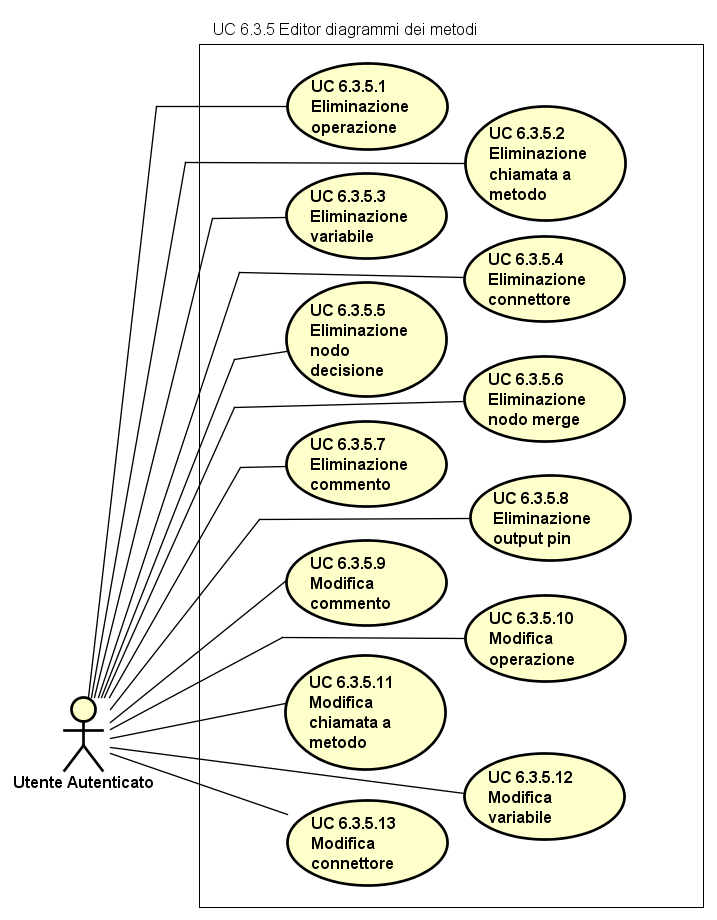
\includegraphics[scale=0.5]{../../Casi D'uso/UC6.3.5.png} 
\caption{Caso d'uso UC6.3.5} 
 \end{figure} 
\begin{itemize} 
\item \textbf{Attori}: Utente autenticato;
\item \textbf{Descrizione}: L'attore può modificare il diagramma del metodo di una classe;
\item \textbf{Precondizione}: Nell'applicazione è caricato correttamente un progetto che  contiene almeno una classe con un metodo, è visualizzata la finestra di modifica del metodo;
\item \textbf{Postcondizione}: Il diagramma del metodo di una classe viene cambiato dalle eventuali modifiche dell'attore;
\item \textbf{Scenario principale}: \begin{enumerate}\item Eliminazione operazione (UC6.3.5.1);\item Modifica operazione (UC6.3.5.10);\item Modifica chiamata a metodo (UC6.3.5.11);\item Modifica variabile (UC6.3.5.12);\item Modifica connettore (UC6.3.5.13);\item Eliminazione chiamata a metodo (UC6.3.5.2);\item Eliminazione variabile (UC6.3.5.3);\item Eliminazione connettore (UC6.3.5.4);\item Eliminazione nodo decisione (UC6.3.5.5);\item Eliminazione nodo merge (UC6.3.5.6);\item Eliminazione commento (UC6.3.5.7);\item Eliminazione output pin (UC6.3.5.8);\item Modifica commento (UC6.3.5.9). 
 \end{enumerate}
\end{itemize} 
\subsection{UC6.3.5.1 - Eliminazione operazione} 
\label{ssec:UC6.3.5.1} 
\begin{itemize} 
\item \textbf{Attori}: Utente autenticato;
\item \textbf{Descrizione}: L'attore può eliminare un elemento operazione fra gli elementi del digramma del metodo di una classe;
\item \textbf{Precondizione}: È visualizzato il diagramma di un metodo che contiene almeno un elemento operazione;
\item \textbf{Postcondizione}: Viene eliminato, dal diagramma del metodo,  l'elemento operazione selezionato dall'attore.
\end{itemize} 
\subsection{UC6.3.5.10 - Modifica operazione} 
\label{ssec:UC6.3.5.10} 
\begin{itemize} 
\item \textbf{Attori}: Utente autenticato;
\item \textbf{Descrizione}: L'attore ha la possibilità di modificare un elemento operazione presente nel diagramma del metodo di una classe;
\item \textbf{Precondizione}: È visualizzato il diagramma di un metodo che contiene almeno un elemento operazione;
\item \textbf{Postcondizione}: Viene modificato l'elemento operazione con i cambiamenti apportati dall'utente;
\item \textbf{Scenario principale}: \begin{enumerate}\item Definizione operazione (UC6.3.5.10.1). 
 \end{enumerate}
\end{itemize} 
\subsection{UC6.3.5.10.1 - Definizione operazione} 
\label{ssec:UC6.3.5.10.1} 
\begin{itemize} 
\item \textbf{Attori}: Utente autenticato;
\item \textbf{Descrizione}: L'attore ha la possibilità di definire un'operazione tramite input testuale;
\item \textbf{Precondizione}: È aperta la finestra di modifica di un elemento operazione;
\item \textbf{Postcondizione}: È applicata l'operazione definita dall'utente.
\end{itemize} 
\subsection{UC6.3.5.11 - Modifica chiamata a metodo} 
\label{ssec:UC6.3.5.11} 
\begin{itemize} 
\item \textbf{Attori}: Utente autenticato;
\item \textbf{Descrizione}: L'attore può modificare l'elemento chiamata a metodo di un diagramma del metodo di una classe;
\item \textbf{Precondizione}: È visualizzato il diagramma di un metodo che contiene almeno un elemento chiamata a metodo;
\item \textbf{Postcondizione}: L'elemento chiamata a metodo viene modificato con le modifiche apportate dall'attore;
\item \textbf{Scenario principale}: \begin{enumerate}\item Selezione metodo (UC6.3.5.11.1). 
 \end{enumerate}
\end{itemize} 
\subsection{UC6.3.5.11.1 - Selezione metodo} 
\label{ssec:UC6.3.5.11.1} 
\begin{itemize} 
\item \textbf{Attori}: Utente autenticato;
\item \textbf{Descrizione}: L'attore può selezionare un metodo dalla lista dei metodi, e parametri in ingresso da esso richiesti;
\item \textbf{Precondizione}: La finestra di modifica di un elemento chiamata a metodo è visualizzata correttamente;
\item \textbf{Postcondizione}: Viene assegnato il metodo, selezionato dall'attore, all'elemento chiamata a metodo e eventuali parametri richiesti.
\end{itemize} 
\subsection{UC6.3.5.12 - Modifica variabile} 
\label{ssec:UC6.3.5.12} 
\begin{itemize} 
\item \textbf{Attori}: Utente autenticato;
\item \textbf{Descrizione}: L'attore può modificare l'elemento variabile di un diagramma del metodo di una classe;
\item \textbf{Precondizione}: È visualizzato il diagramma di un metodo che contiene almeno un elemento variabile;
\item \textbf{Postcondizione}: L'elemento variabile viene modificato con le modifiche apportate dall'attore;
\item \textbf{Scenario principale}: \begin{enumerate}\item Istanziazione nuova variabile (UC6.3.5.12.1). 
 \end{enumerate}
\end{itemize} 
\subsection{UC6.3.5.12.1 - Istanziazione nuova variabile} 
\label{ssec:UC6.3.5.12.1} 
\begin{itemize} 
\item \textbf{Attori}: Utente autenticato;
\item \textbf{Descrizione}: L'attore può definire una nuova variabile per l'elemento variabile corrente;
\item \textbf{Precondizione}: Viene visualizzata correttamente la finestra di modifica dell'elemento variabile;
\item \textbf{Postcondizione}: È applicata, all'elemento variabile, la variabile definita dall'attore.
\end{itemize} 
\subsection{UC6.3.5.13 - Modifica connettore} 
\label{ssec:UC6.3.5.13} 
\begin{itemize} 
\item \textbf{Attori}: Utente autenticato;
\item \textbf{Descrizione}: L'attore può operare delle modifiche su un elemento connettore presente nel diagramma del metodo di una classe;
\item \textbf{Precondizione}: È visualizzato il diagramma di un metodo che contiene almeno un elemento connettore;
\item \textbf{Postcondizione}: Vengono applicate le modifiche eventualmente apportate dall'attore;
\item \textbf{Scenario principale}: \begin{enumerate}\item Definizione condizione di guardia (UC6.3.5.13.1). 
 \end{enumerate}
\end{itemize} 
\subsection{UC6.3.5.13.1 - Definizione condizione di guardia} 
\label{ssec:UC6.3.5.13.1} 
\begin{itemize} 
\item \textbf{Attori}: Utente autenticato;
\item \textbf{Descrizione}: L'attore può definire una guardia per l'elemento connettore;
\item \textbf{Precondizione}: Viene visualizzata la finestra di modifica dell'elemento connettore;
\item \textbf{Postcondizione}: Viene ridefinita la guardia come specificato dall'attore.
\end{itemize} 
\subsection{UC6.3.5.2 - Eliminazione chiamata a metodo} 
\label{ssec:UC6.3.5.2} 
\begin{itemize} 
\item \textbf{Attori}: Utente autenticato;
\item \textbf{Descrizione}: L'attore può eliminare, dal diagramma del metodo di una classe, un elemento chiamata a metodo;
\item \textbf{Precondizione}: È visualizzato il diagramma di un metodo che contiene almeno un elemento chiamata a metodo;
\item \textbf{Postcondizione}: Viene eliminato, dal diagramma del metodo,  l'elemento chiamata a metodo selezionato dall'attore.
\end{itemize} 
\subsection{UC6.3.5.3 - Eliminazione variabile} 
\label{ssec:UC6.3.5.3} 
\begin{itemize} 
\item \textbf{Attori}: Utente autenticato;
\item \textbf{Descrizione}: L'attore può eliminare un elemento variabile presente nel diagramma del metodo di una classe;
\item \textbf{Precondizione}: È visualizzato il diagramma di un metodo che contiene almeno un elemento variabile;
\item \textbf{Postcondizione}: Viene eliminato, dal diagramma del metodo,  l'elemento variabile selezionato dall'attore.
\end{itemize} 
\subsection{UC6.3.5.4 - Eliminazione connettore} 
\label{ssec:UC6.3.5.4} 
\begin{itemize} 
\item \textbf{Attori}: Utente autenticato;
\item \textbf{Descrizione}: L'attore può eliminare, dal diagramma del metodo di una classe, un elemento connettore;
\item \textbf{Precondizione}: È visualizzato il diagramma di un metodo che contiene almeno un elemento connettore;
\item \textbf{Postcondizione}: Viene eliminato, dal diagramma del metodo,  l'elemento chiamata a metodo selezionato dall'attore.
\end{itemize} 
\subsection{UC6.3.5.5 - Eliminazione nodo decisione} 
\label{ssec:UC6.3.5.5} 
\begin{itemize} 
\item \textbf{Attori}: Utente autenticato;
\item \textbf{Descrizione}: L'attore ha la possibilità di eliminare un elemento nodo decisione dal diagramma del metodo di una classe;
\item \textbf{Precondizione}: È visualizzato il diagramma di un metodo che contiene almeno un elemento nodo decisione;
\item \textbf{Postcondizione}: Viene eliminato, dal diagramma del metodo,  l'elemento nodo decisione selezionato dall'attore.
\end{itemize} 
\subsection{UC6.3.5.6 - Eliminazione nodo merge} 
\label{ssec:UC6.3.5.6} 
\begin{itemize} 
\item \textbf{Attori}: Utente autenticato;
\item \textbf{Descrizione}: L'attore può eliminare, dal diagramma del metodo di una classe, un elemento nodo merge;
\item \textbf{Precondizione}: È visualizzato il diagramma di un metodo che contiene almeno un elemento nodo merge;
\item \textbf{Postcondizione}: Viene eliminato, dal diagramma del metodo,  l'elemento nodo merge selezionato dall'attore.
\end{itemize} 
\subsection{UC6.3.5.7 - Eliminazione commento} 
\label{ssec:UC6.3.5.7} 
\begin{itemize} 
\item \textbf{Attori}: Utente autenticato;
\item \textbf{Descrizione}: L'attore può eliminare, dal diagramma del metodo di una classe, un elemento commento;
\item \textbf{Precondizione}: È visualizzato il diagramma di un metodo che contiene almeno un elemento commento;
\item \textbf{Postcondizione}: Viene eliminato, dal diagramma del metodo,  l'elemento commento selezionato dall'attore.
\end{itemize} 
\subsection{UC6.3.5.8 - Eliminazione output pin} 
\label{ssec:UC6.3.5.8} 
\begin{itemize} 
\item \textbf{Attori}: Utente autenticato;
\item \textbf{Descrizione}: L'attore può eliminare, dal diagramma del metodo di una classe, un elemento output pin;
\item \textbf{Precondizione}: È visualizzato il diagramma di un metodo che contiene almeno un elemento output pin;
\item \textbf{Postcondizione}: L'elemento output pin, selezionato dall'utente, viene rimosso dal diagramma del metodo.
\end{itemize} 
\subsection{UC6.3.5.9 - Modifica commento} 
\label{ssec:UC6.3.5.9} 
\begin{itemize} 
\item \textbf{Attori}: Utente autenticato;
\item \textbf{Descrizione}: L'attore può modificare un elemento commento presente nel diagramma del metodo di una classe;
\item \textbf{Precondizione}: È visualizzato il diagramma di un metodo che contiene almeno un elemento commento;
\item \textbf{Postcondizione}: Vengono apportate le modifiche, all'elemento commento, effettuate dall'attore.
\end{itemize} 
\newpage
\subsection{UC6.4 - Pannello laterale} 
\label{ssec:UC6.4}

\begin{figure}[h!] 
\centering 
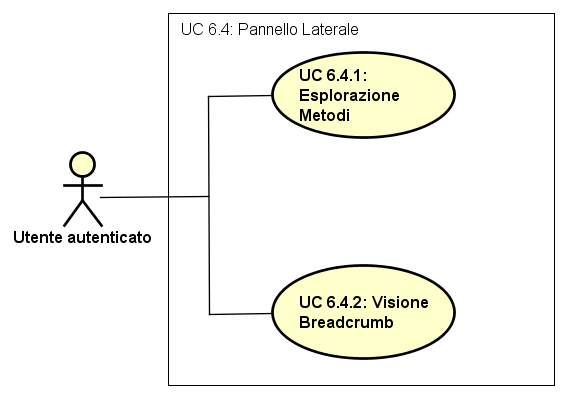
\includegraphics[scale=0.5]{../../Casi D'uso/UC6.4.png} 
\caption{Caso d'uso UC6.4} 
 \end{figure} 
\begin{itemize} 
\item \textbf{Attori}: Utente autenticato;
\item \textbf{Descrizione}: L'attore può accedere a questa sezione di schermo nella quale è possibile visionare il flusso del programma a partire dal metodo main;
\item \textbf{Precondizione}: È aperto un progetto;
\item \textbf{Postcondizione}: Visualizza un diagramma delle attività;
\item \textbf{Scenario principale}: \begin{enumerate}\item Esplorazione metodi (UC6.4.1);\item Visione Breadcrumb (UC6.4.2). 
 \end{enumerate}
\end{itemize} 
\subsection{UC6.4.1 - Esplorazione metodi} 
\label{ssec:UC6.4.1} 
\begin{itemize} 
\item \textbf{Attori}: Utente autenticato;
\item \textbf{Descrizione}: L'attore, selezionando una chiamata a metodo, può visionare il diagramma delle attività di tale metodo;
\item \textbf{Precondizione}: È visualizzato un diagramma delle attività;
\item \textbf{Postcondizione}: Viene mostrato il diagramma delle attività del metodo selezionato.
\end{itemize} 
\subsection{UC6.4.2 - Visione Breadcrumb} 
\label{ssec:UC6.4.2} 
\begin{itemize} 
\item \textbf{Attori}: Utente autenticato;
\item \textbf{Descrizione}: Viene visualizzata una Breadcrumb che rappresenta il percorso effettuato dall'utente durante la navigazione dei vari metodo selezionati;
\item \textbf{Precondizione}: E' visualizzato un diagramma delle attività;
\item \textbf{Postcondizione}: Vengono visualizzati in ordine di accesso tutti i metodi selezionati dall'utente nella visione principale del programma.
\end{itemize} 
